% Template setup and packages.
\documentclass[10pt,landscape,a4paper]{article}
\usepackage{multicol}
\usepackage{calc}
\usepackage{ifthen}
\usepackage{geometry}

% Custom packages.
\usepackage{amsmath}
\usepackage{mathtools}
\usepackage{amssymb}
\usepackage{mathrsfs}
\usepackage{stix2}
\usepackage{systeme}
\usepackage{graphicx}
\usepackage{float}
\usepackage{physics}
\usepackage{siunitx}
\usepackage{collcell} % loads array
\newcolumntype{M}{>{$} l <{$}}
\newcolumntype{U}{>{$[\collectcell\si} l <{\endcollectcell]$}}

% Hyperref. Remember to change title!
\usepackage{hyperref}
\hypersetup{pdfauthor={Teemu Weckroth},pdftitle={Signals and Systems}}

% Path to graphics folder.
\graphicspath{ {./figures/} }

% Change fonts for v and w.
\DeclareSymbolFont{txletters}{OML}{ntxmi}{m}{it}
\SetSymbolFont{txletters}{bold}{OML}{ntxmi}{b}{it}
\DeclareFontSubstitution{OML}{ntxmi}{m}{it}
\DeclareMathSymbol{v}{\mathalpha}{txletters}{`v}
\DeclareMathSymbol{w}{\mathalpha}{txletters}{`w}

% Must be below font changes to avoid errors.
\usepackage{bm}

% Commands for differentials. Redefines the underdot command!
\renewcommand\d{\mathop{}\!\mathrm{d}}
\newcommand\p{\mathop{}\!\mathrm{\partial}}
%\newcommand\e{\mathrm{e}}

% Commands for the set of real numbers and Lagrangian/Laplace.
\newcommand{\R}{\mathbb{R}}
\newcommand{\La}{\mathscr{L}}

\DeclareMathOperator{\sinc}{sinc}
\newcommand{\F}{\mathscr{F}}

% Unbreakable unit environment.
\newenvironment{absolutelynopagebreak}
{\par\nobreak\vfil\penalty0\vfilneg
	\vtop\bgroup}
{\par\xdef\tpd{\the\prevdepth}\egroup
	\prevdepth=\tpd}

% Shrink bullet points.
\renewcommand\labelitemi{$\vcenter{\hbox{\tiny$\bullet$}}$}

%
\ifthenelse{\lengthtest { \paperwidth = 11in}}
{ \geometry{top=.5in,left=.5in,right=.5in,bottom=.5in} }
{\ifthenelse{ \lengthtest{ \paperwidth = 297mm}}
	{\geometry{top=1cm,left=1cm,right=1cm,bottom=1cm} }
	{\geometry{top=1cm,left=1cm,right=1cm,bottom=1cm} }
}

% Turn off header and footer
\pagestyle{empty}

% Redefine section commands to use less space
\makeatletter
\renewcommand{\section}{\@startsection{section}{1}{0mm}%
	{-1ex plus -.5ex minus -.2ex}%
	{0.5ex plus .2ex}%x
	{\normalfont\large\bfseries}}
\renewcommand{\subsection}{\@startsection{subsection}{2}{0mm}%
	{-1explus -.5ex minus -.2ex}%
	{0.5ex plus .2ex}%
	{\normalfont\normalsize\bfseries}}
\renewcommand{\subsubsection}{\@startsection{subsubsection}{3}{0mm}%
	{-1ex plus -.5ex minus -.2ex}%
	{1ex plus .2ex}%
	{\normalfont\small\bfseries}}
\makeatother

% Define BibTeX command
\def\BibTeX{{\rm B\kern-.05em{\sc i\kern-.025em b}\kern-.08em
		T\kern-.1667em\lower.7ex\hbox{E}\kern-.125emX}}

% Don't print section numbers
\setcounter{secnumdepth}{0}

\setlength{\parindent}{0pt}
\setlength{\parskip}{0pt plus 0.5ex}

\begin{document}
	
	\raggedright
	\footnotesize
	\begin{multicols}{3}
		% multicol parameters
		% These lengths are set only within the two main columns
		%\setlength{\columnseprule}{0.25pt}
		\setlength{\premulticols}{1pt}
		\setlength{\postmulticols}{1pt}
		\setlength{\multicolsep}{1pt}
		\setlength{\columnsep}{2pt}
		
		\part*{Signals and Systems.}
		\begin{center}
			Teemu Weckroth, \today
		\end{center}
		
		\section{Complex numbers.}
			\begin{align*}
				j \vcentcolon &= \sqrt{-1}\\
				e^{j a} &= \cos{a} + j \sin{a}\\
				z &= a + jb = r \cdot e^{j \theta}\\
				z^* &= a - j b = r \cdot e^{- j \theta}\\
				r &= \sqrt{a^2 + b^2}\\
				\theta &= \arctan\left( \frac{b}{a}\right)\\
				a &= r \cdot \cos{\theta}\\
				b &= r \cdot \sin{\theta}
			\end{align*}
		For special case $r = 1$:
			\begin{align*}
				z &= e^{j \theta} = \cos{\theta} + j \sin{\theta}\\
				z^{*} &= e^{- j \theta} = \cos{\theta} - j \sin{\theta}\\
				\cos{\theta} &= \frac{1}{2} \left(e^{j \theta} + e^{- j \theta}\right)\\
				\sin{\theta} &= \frac{1}{2j} \left(e^{j \theta} - e^{- j \theta}\right)
			\end{align*}
		
		\section{Operations with complex numbers.}
		Take $z_1 = a_1 + j b_1 = r_1 e^{j \theta_1}$ and $z_2 = a_2 + j b_2 = r_2 e^{j \theta_2}$:
			\begin{align*}
				z_1 + z_2 &= (a_1 + b_2) + j(b_1 + b_2)\\
				z_1 \cdot z_2 &= (a_1 a_2 - b_1 b_2) + j(a_1 b_2 + a_1 b_2)\\
				&= r_1 r_2 e^{j(\theta_1 + \theta_2)}\\
				\frac{1}{z_1} &= \frac{1}{a_1 + j b_1} = \frac{1}{r_1} e^{- j \theta_1}\\
				\frac{z_2}{z_1} &= \frac{r_2}{r_1} e^{j(\theta_2 - \theta_1)}\\
				{\lvert z_1 \rvert}^2 &= z_1 \cdot z_1^*
			\end{align*}
		
		\section{Harmonic functions and phasors.}
		We often deal with signals of the form
		\[
			x_a (t) = A \cos{(\omega t + \phi)}
		\]
		or
		\[
			x_b (t) = A_1 \cos{(\omega t + \phi_1)} + A_2 \cos{(\omega t + \phi_2)}
		\]
		We can write $x_a (t)$ as
		\[
			x_a (t) = \Re(A e^{j(\omega t + \phi)}) = \Re(e^{j \omega t} \cdot A e^{j \phi})
		\]
		and $x_b (t))$ as
		\[
			x_b (t) = \Re(e^{j \omega t} \cdot (A_1 e^{j \phi_1} + A_2 e^{j \phi_2}))
		\]
		
		\section{Signal with delay.}
		Signal $y(t)$ delayed by $\tau$ can be written as
		\[
			y(t) = k \cdot x(t - \tau)
		\]
		or as a convolution
		\[
			y(t) = x(t) * h(t)
		\]
		with
		\[
			h(t) = k \cdot \delta (t - \tau)
		\]
		
		\section{Moving average.}
		The signal can be written as
		\[
			y(t) = k \cdot \frac{1}{T_0} \int_{t-T_0}^{t}{x(\alpha) \cdot d\alpha}
		\]
		or as a convolution
		\[
			y(t) = x(t) * h(t)
		\]
		with
		\[
			h(t) = \frac{k}{T_0} \Pi\left({\frac{t - T_0/2}{T_0}}\right)
		\]
		
		\section{Unit step function $ u(t) $.}
		Describes something starting at $t=0$:
		\[
			u(t) = \begin{cases}
				0 &\text{for}~t < 0\\
				1 &\text{for}~t \geq 0
			\end{cases}
		\]
		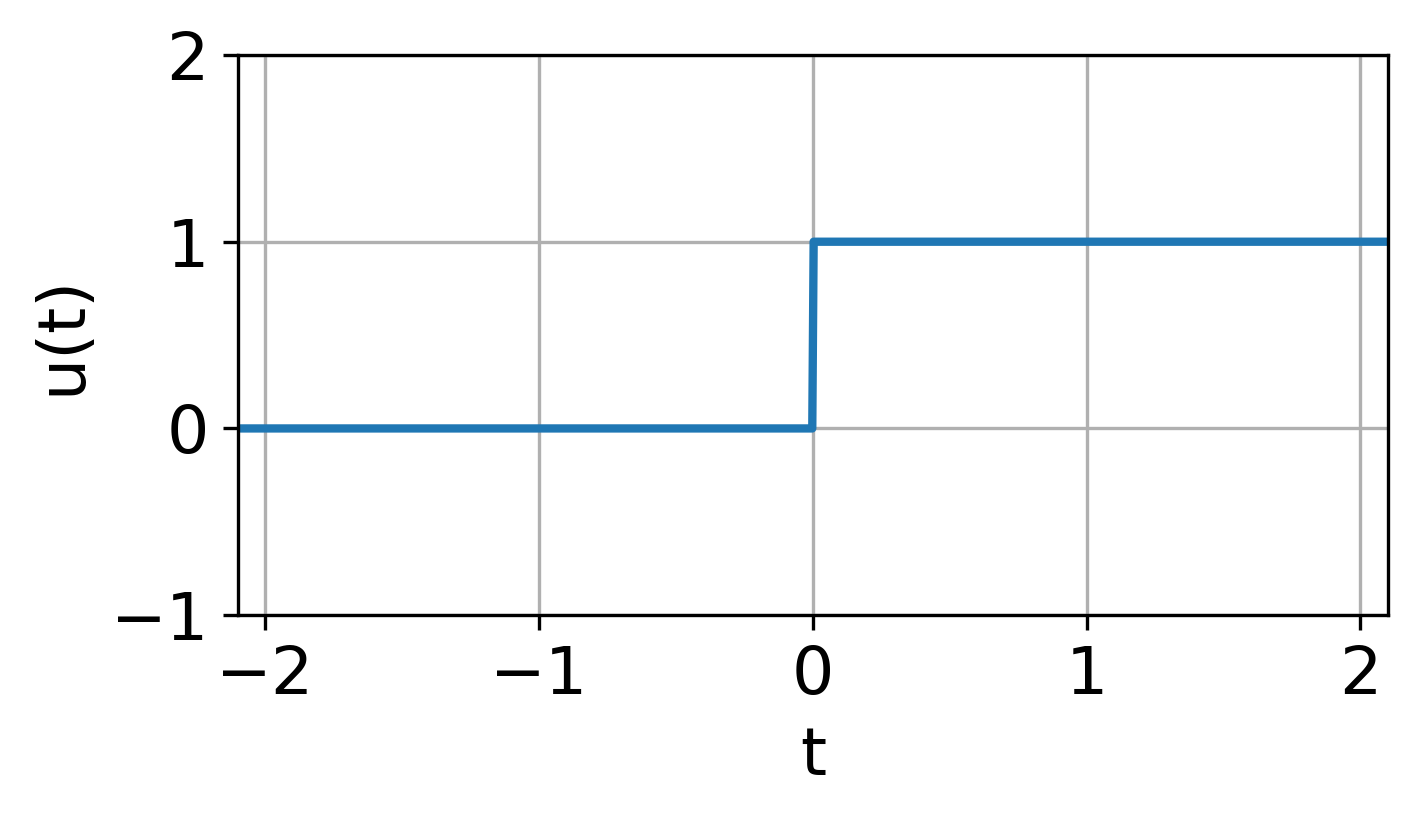
\includegraphics[width=\textwidth/5]{step_function}
		
		\section{Unit pulse function $ \Pi(t) $.}
		Describes something lasting for one second and centred at $t=0$:
		\[
			\Pi(t) = \begin{cases}
				1 &\text{for}~\lvert t \rvert \leq \frac{1}{2}\\
				0 &\text{elsewhere}
			\end{cases}
		\]
		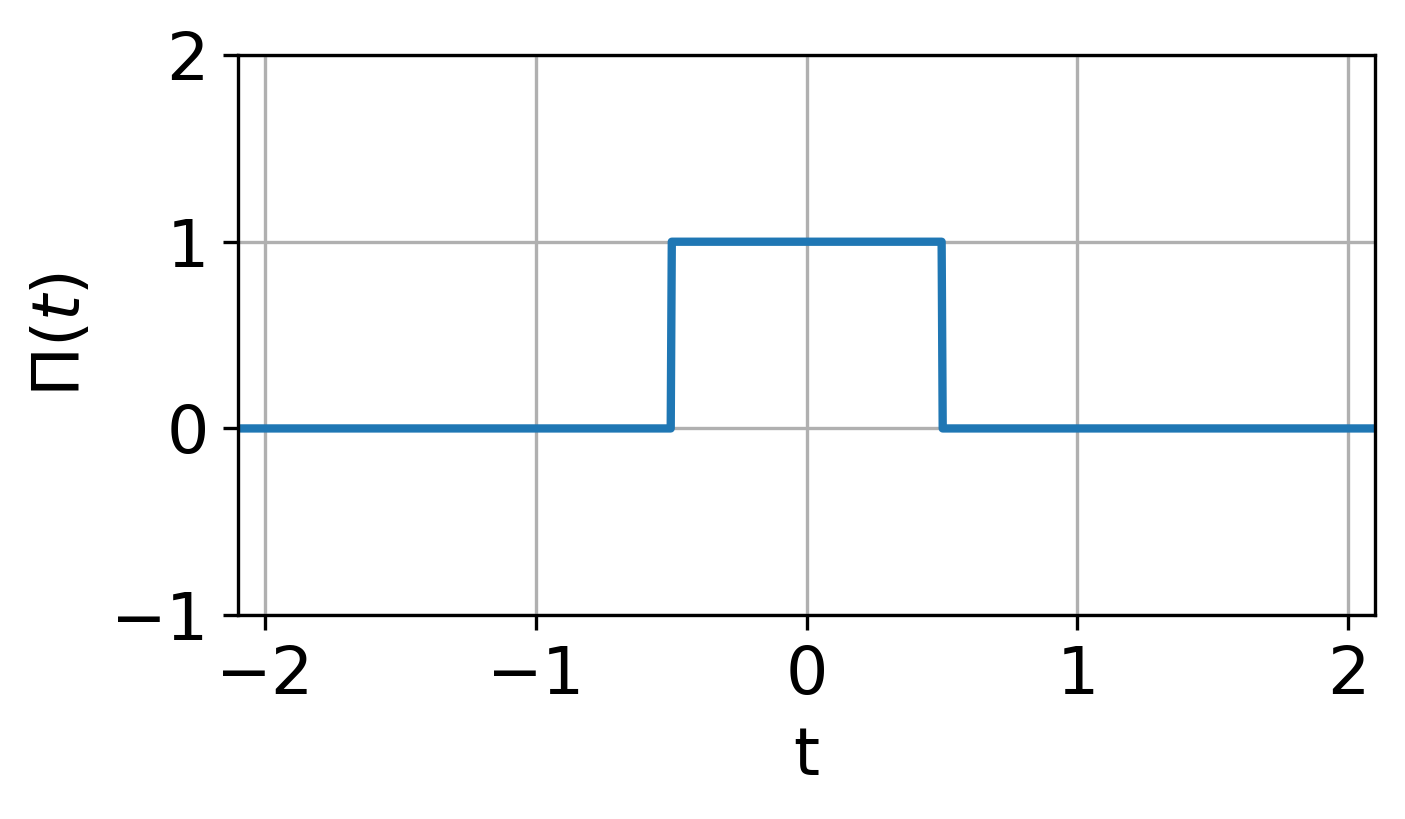
\includegraphics[width=\textwidth/5]{unitpulse_function}
		
		\section{Discrete-time unit impulse $ \delta[n] $.}
		Describes something lasting for one sample and centred at $n=0$:
		\[
			\delta[n] = \begin{cases}
				1 &\text{for}~n=0\\
				0 &\text{elsewhere}
			\end{cases}
		\]
		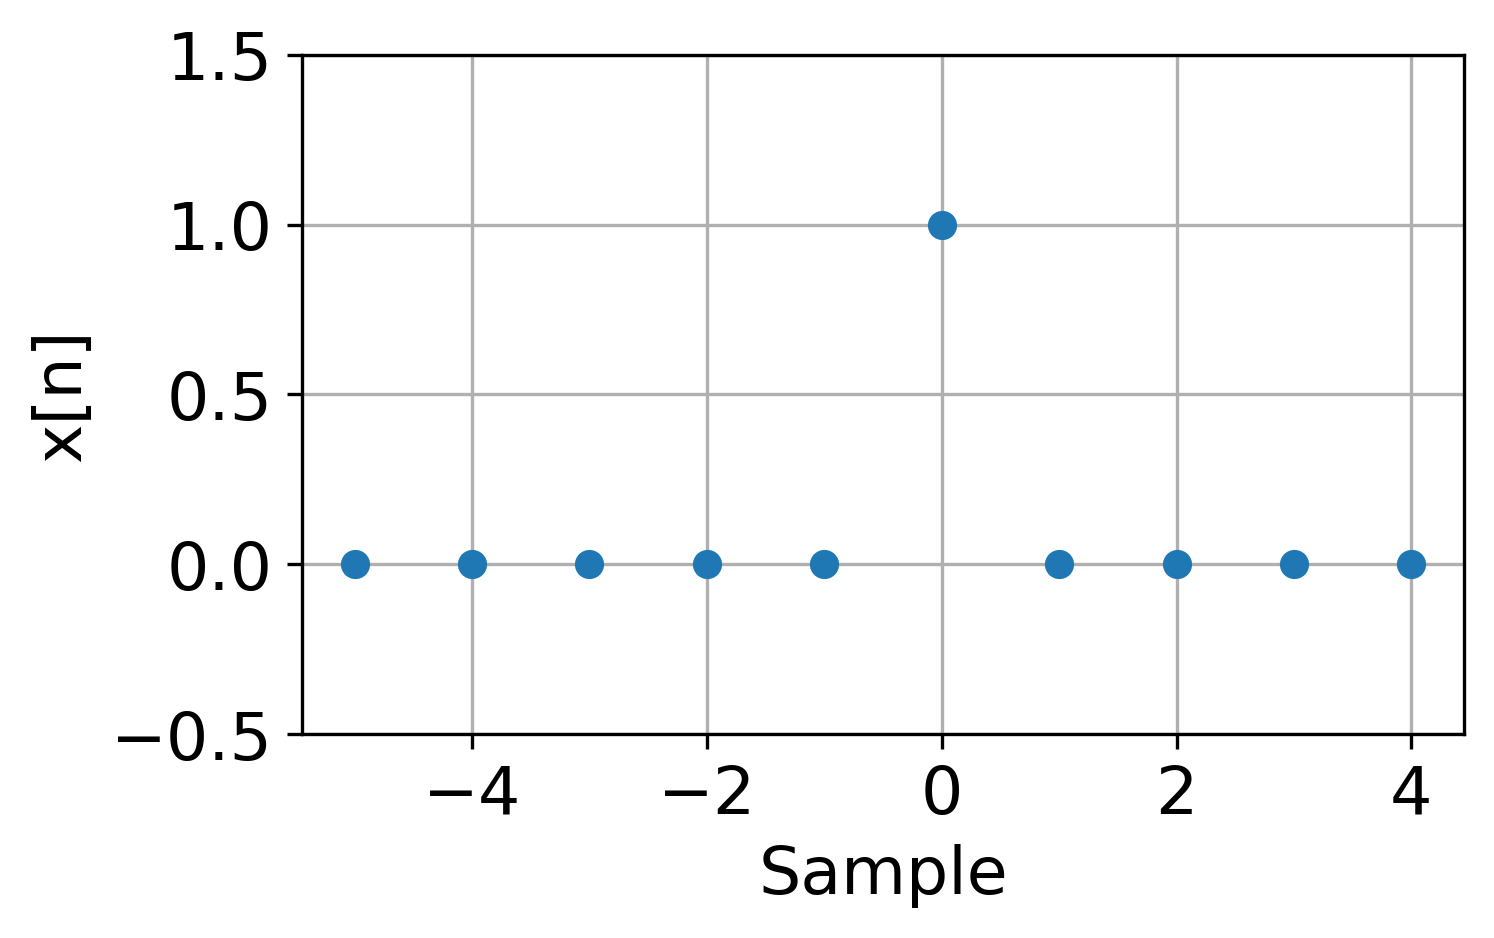
\includegraphics[width=\textwidth/5]{discrete_impulse}
		
		\section{Sinc function $ \sinc(t) $.}
		\[
			\sinc(t) = \frac{\sin{(\pi \cdot t)}}{\pi \cdot t}
		\]
		Sampling the $\sinc$ function with sampling intervals $T_s = 1$ gives us the discrete unit pulse $\delta[n] = \sinc(1 \cdot n)$.
		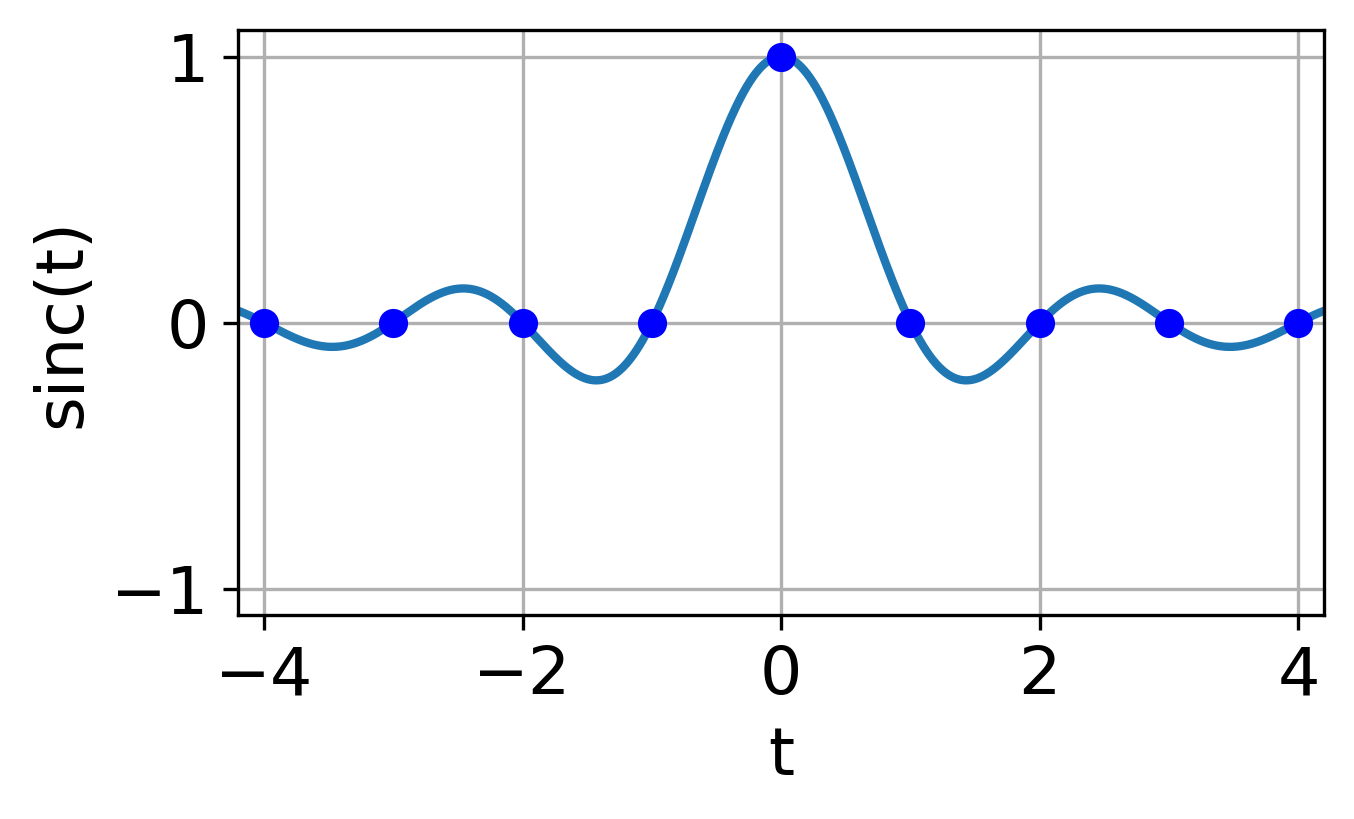
\includegraphics[width=\textwidth/5]{sinc_sampled}
		
		\section{Triangle function $ \Lambda \left(\frac{t}{T}\right) $.}
		\[
			\Lambda \left(\frac{t}{T}\right) = \begin{cases}
				1 - \left|\frac{t}{T}\right| &~\text{for}~t\in [-T,T]\\
				0 &~\text{elsewhere}
			\end{cases}
		\]
		We encounter this while studying the convolution
		\[
			\frac{1}{T} \cdot \Pi \left(\frac{t}{T}\right) \ast \Pi \left(\frac{t}{T}\right) = \Lambda \left(\frac{t}{T}\right)
		\]
		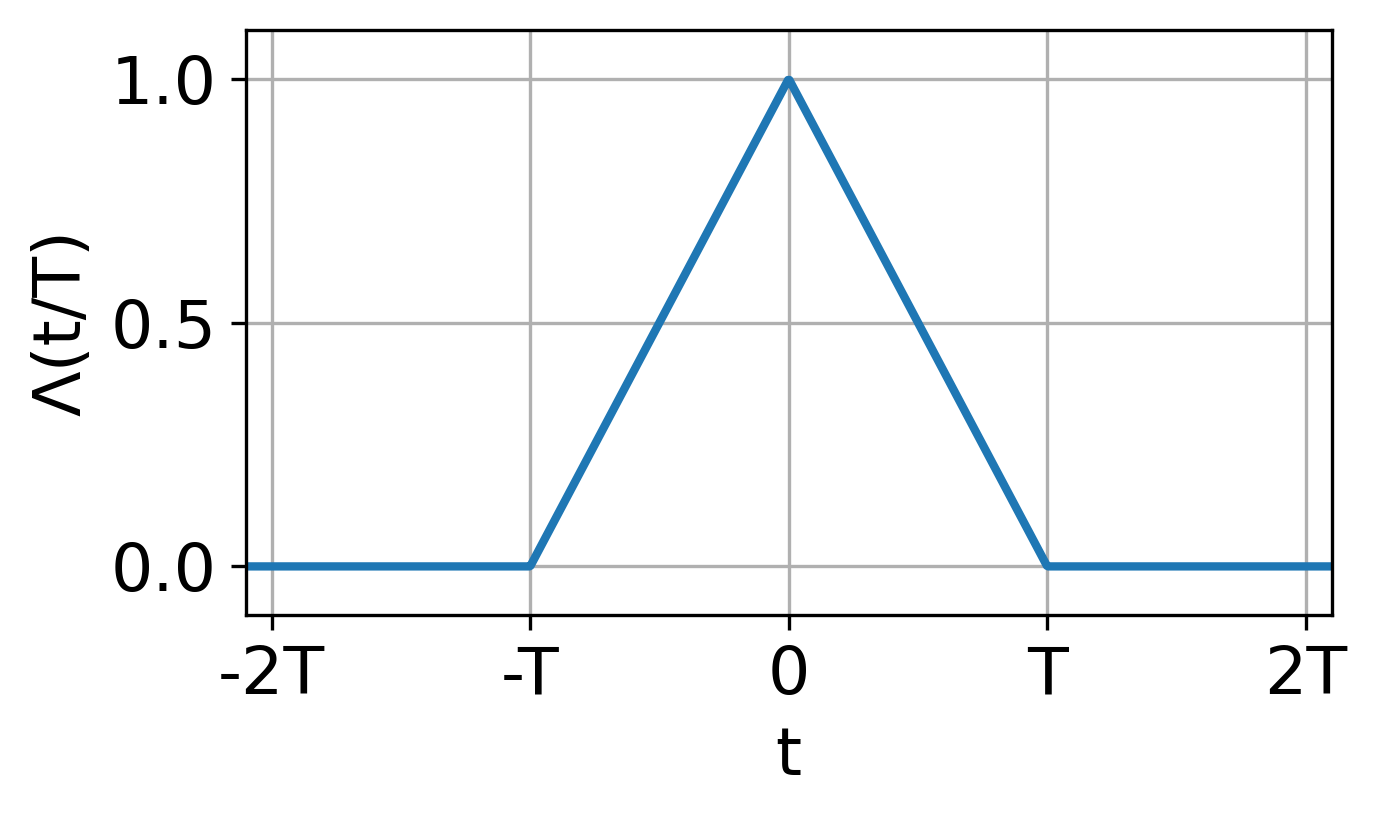
\includegraphics[width=\textwidth/5]{triangle_function}
		
		\section{Periodic signals.}
		Periodic signals repeat after period $T_0 = \frac{1}{f_0} = \frac{2\pi}{\omega_0}$:
		\[
			x(t) = x(t + T_0) = x(t + n \cdot T_0)
		\]
		
		\section{Phasors.}
		Take
		\[
			x(t) = 2 \cdot \cos{\left(2\pi \cdot 10 \cdot t + \frac{\pi}{4}\right)}
		\]
		Using Euler's theorem:
			\begin{align*}
				x(t) &= \Re{\left(2 \cdot e^{j(2\pi \cdot 10 \cdot t + \frac{\pi}{4})}\right)} \\&= \frac{1}{2} \left(2 \cdot e^{j(2\pi \cdot 10 \cdot t + \frac{\pi}{4})} + 2\cdot e^{-j (2\pi \cdot 10 \cdot t + \frac{\pi}{4})}\right)
			\end{align*}
		
		\section{Dirac delta function $\delta(t)$.}
		Properties that define it:
		\[
			\delta(t) = 0~\text{for}~t \neq 0
		\]
		\[
			\int_{-\infty}^{\infty} \delta(t)~dt = 1
		\]
		Consequences:
		\[
			u(t) = \int_{-\infty}^{t} \delta(\tau)~d\tau
		\]
			\begin{align*}
				\int_{-\infty}^{\infty} x(\tau) \cdot \delta(t - \tau)~d\tau &= \int_{-\infty}^{\infty} x(t - \tau) \cdot \delta(\tau)~d\tau\\&= x(t)
			\end{align*}
		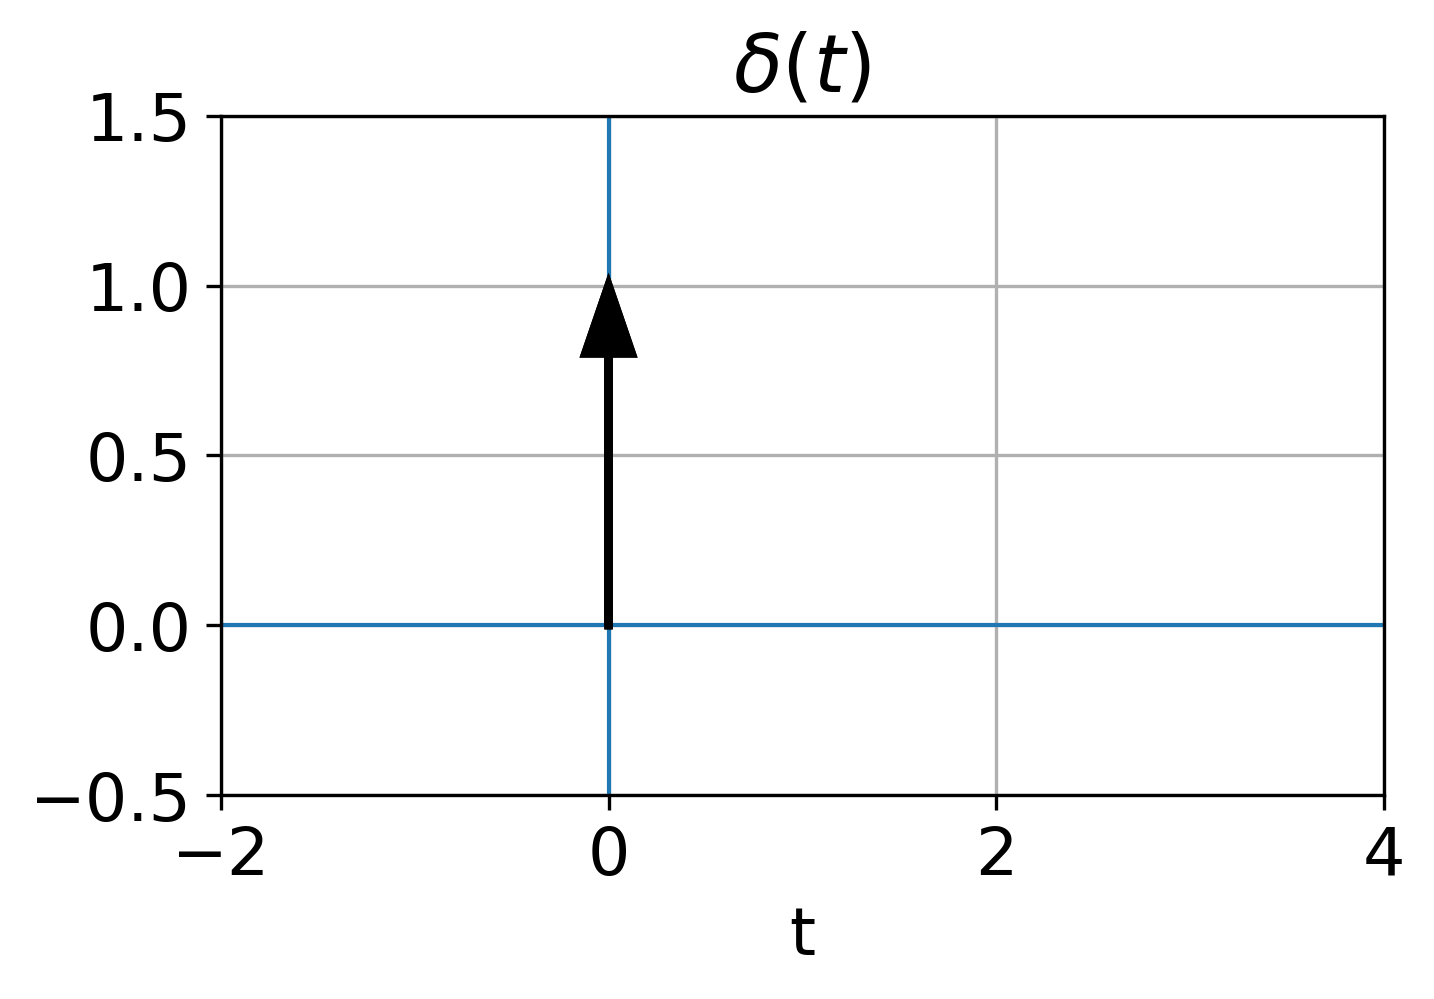
\includegraphics[width=\textwidth/5]{delta_0}
		
		\section{Energy and power of a signal.}
		\[
			E = \int_{-\infty}^{\infty} {\lvert x(t) \rvert}^2~dt
		\]
		Formally it is
		\[
			E = \lim_{T \rightarrow \infty} \int_{-T/2}^{T/2} {\lvert x(t) \rvert}^2~dt
		\]
		For signals with infinite energy:
		\[
			P = \lim_{T \rightarrow \infty} \frac{1}{T} \int_{-T/2}^{T/2} {\lvert x(t) \rvert}^2~dt
		\]
		For periodic signals:
		\[
			P = \frac{1}{T_0} \int_{<T_0>} {\lvert x(t) \rvert}^2~dt
		\]	
		
		\section{Systems defined by simple ODEs.}
		For a system described by
		\[
			\frac{dy(t)}{dt} + k \cdot y(t) = k \cdot x(t)
		\]
		where $x(t) = T_0~u(t)$, the solution $y(t)$ is given by
		\[
			y(t) = T_0 \left(1 - e^{-kt}\right) \cdot u(t)
		\]
		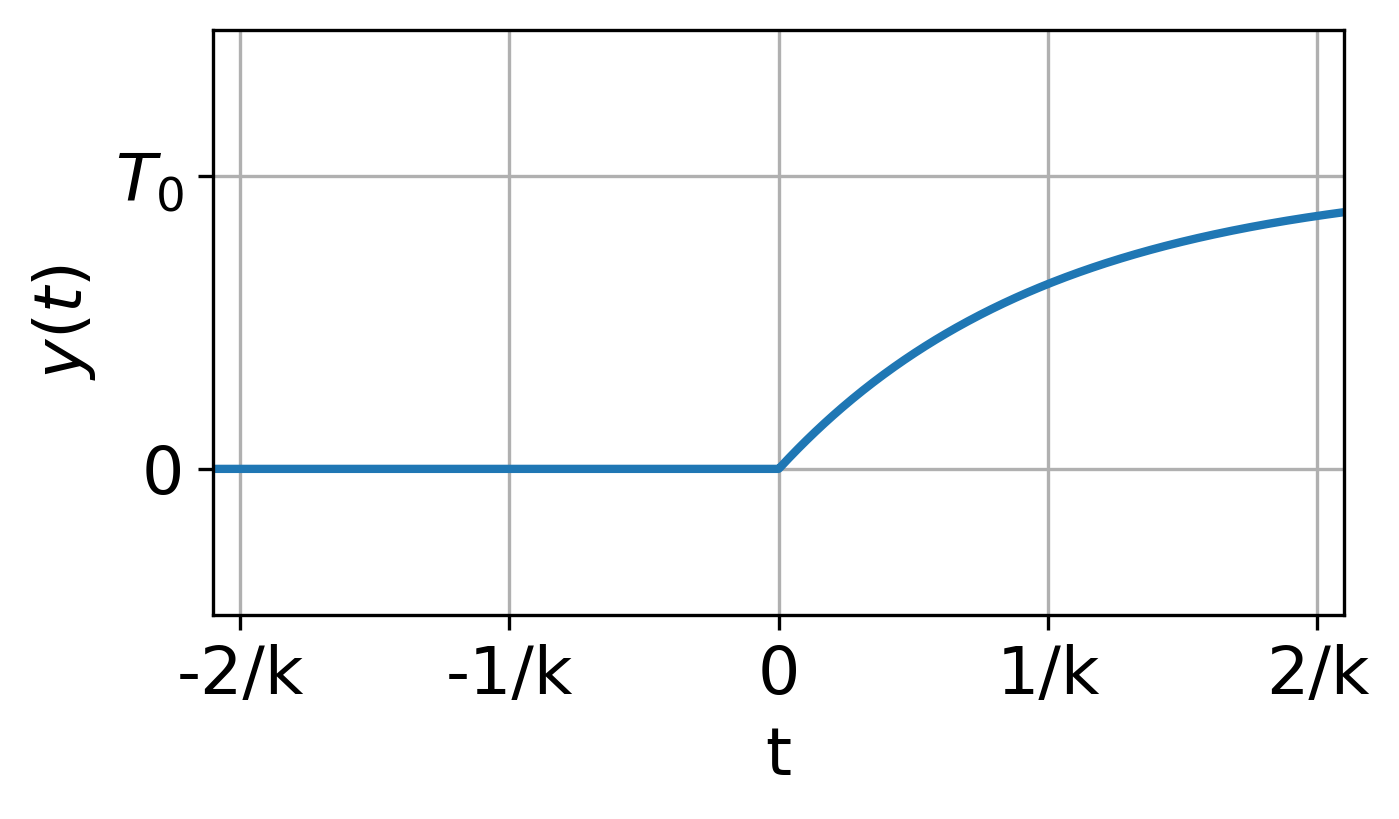
\includegraphics[width=\textwidth/5]{thermo_step_response}
		
		The output of a system where the input is $\delta(n)$ is called the impulse response $h(t)$. In this case:
		\[
			y(t) = h(t) = k \cdot e^{-kt} \cdot u(t)
		\]
		
		\section{Variant vs invariant systems.}
		For a time-invariant system with input-output pair x(t) and y(t) and any time-shift $\tau$:
		\[
			x(t - \tau) \rightarrow \boxed{\text{Time-invariant system}} \rightarrow y(t - \tau)
		\]
		
		\section{Example.}
			\[
				y(t) = \frac{1}{T_0} \cdot \int_{t-T_0}^{t} x(\alpha)~d\alpha
			\]
		Give the input as signal $x_1 (t) = x(t - \tau)$:
			\[
				y_1 (t) = \frac{1}{T_0} \cdot \int_{t-T_0}^{t} x_1(\alpha)~d\alpha
			\]
		Variable change: $\beta = \alpha - \tau$, so that $\alpha = \beta + \tau$ and $d\alpha = d\beta$.\\
		Substitute and change the integration limits:
			\[
				y_1 (t) = \frac{1}{T_0} \cdot \int_{(t - \tau) - T_0}^{(t - \tau)} x(\beta)~d\beta = y(t - \tau)
			\]
		
		\section{Linear systems.}
		A system is linear if, for any constants $a$ and $b$ and inputs $x_1(t)$ and $x_2(t)$:
			\[
				\mathcal{H}[a \cdot x_1(t) + b \cdot x_2(t)] = a \cdot \mathcal{H}[x_1(t)] + b \cdot \mathcal{H}[x_2 (t)]
			\]
		
		\section{Causal systems.}
		A system is causal if the output signal does not depend on future inputs.\\
		Example: $y(t) = \frac{1}{T_0} \cdot \int_{t-T_0}^{t} x(\alpha)~d\alpha$.\\
		Counter-example: $\mathcal{H}[x(t)] = x(t + 1)$, $\mathcal{H}[x(t)] = \frac{1}{T_0} \cdot \int_{t}^{t+T_0} x(\alpha)~d\alpha$.
		
		\section{LTI systems, impulse response, and the convolution.}
		\[
			\delta(t) \rightarrow \boxed{\text{System}} \rightarrow h(t)
		\]
		\[
			x(t) \rightarrow \boxed{\text{System}} \rightarrow \int_{-\infty}^{\infty} x(\tau) \cdot h(t - \tau)~d\tau = x(t) * h(t)
		\]
		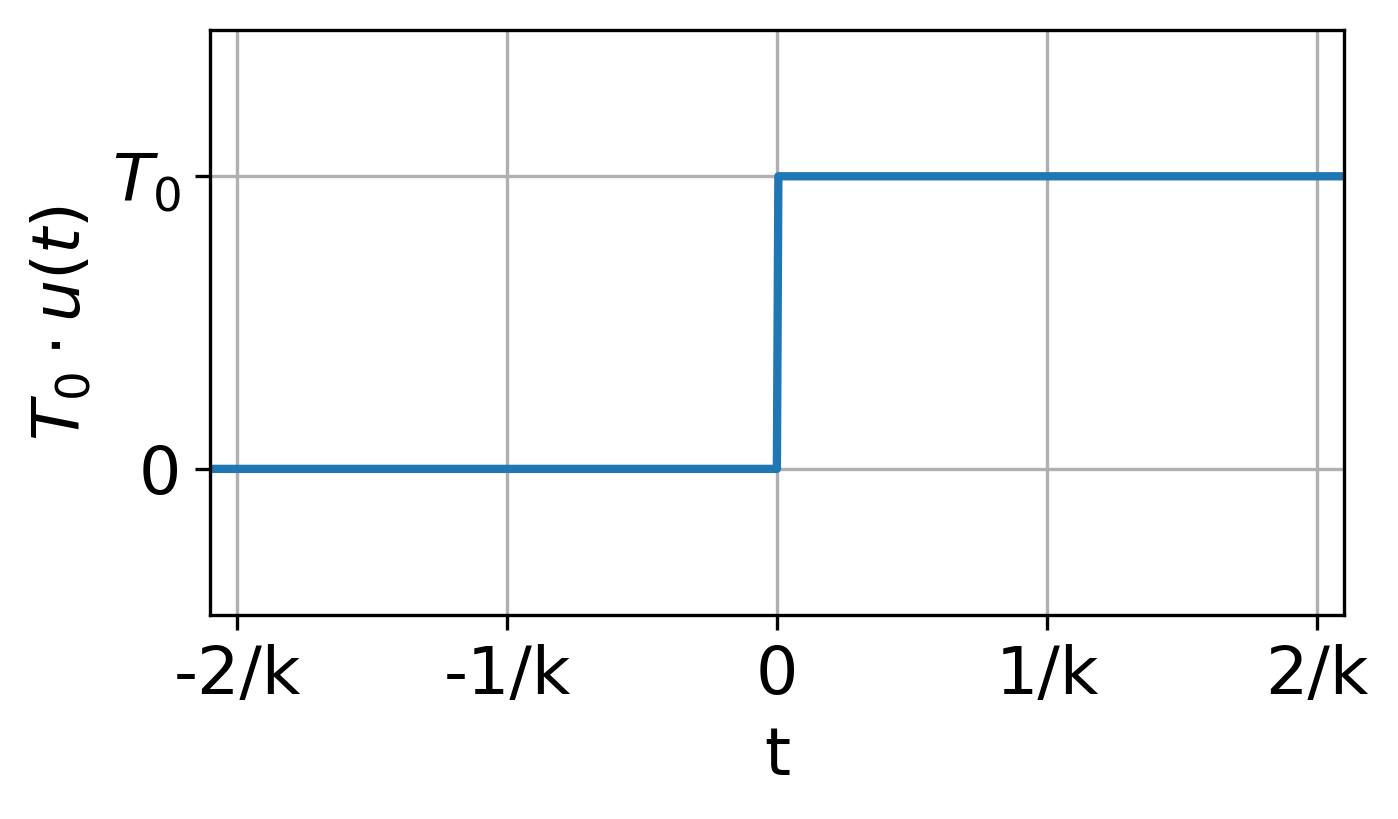
\includegraphics[width=\textwidth/5]{step_temperature}
		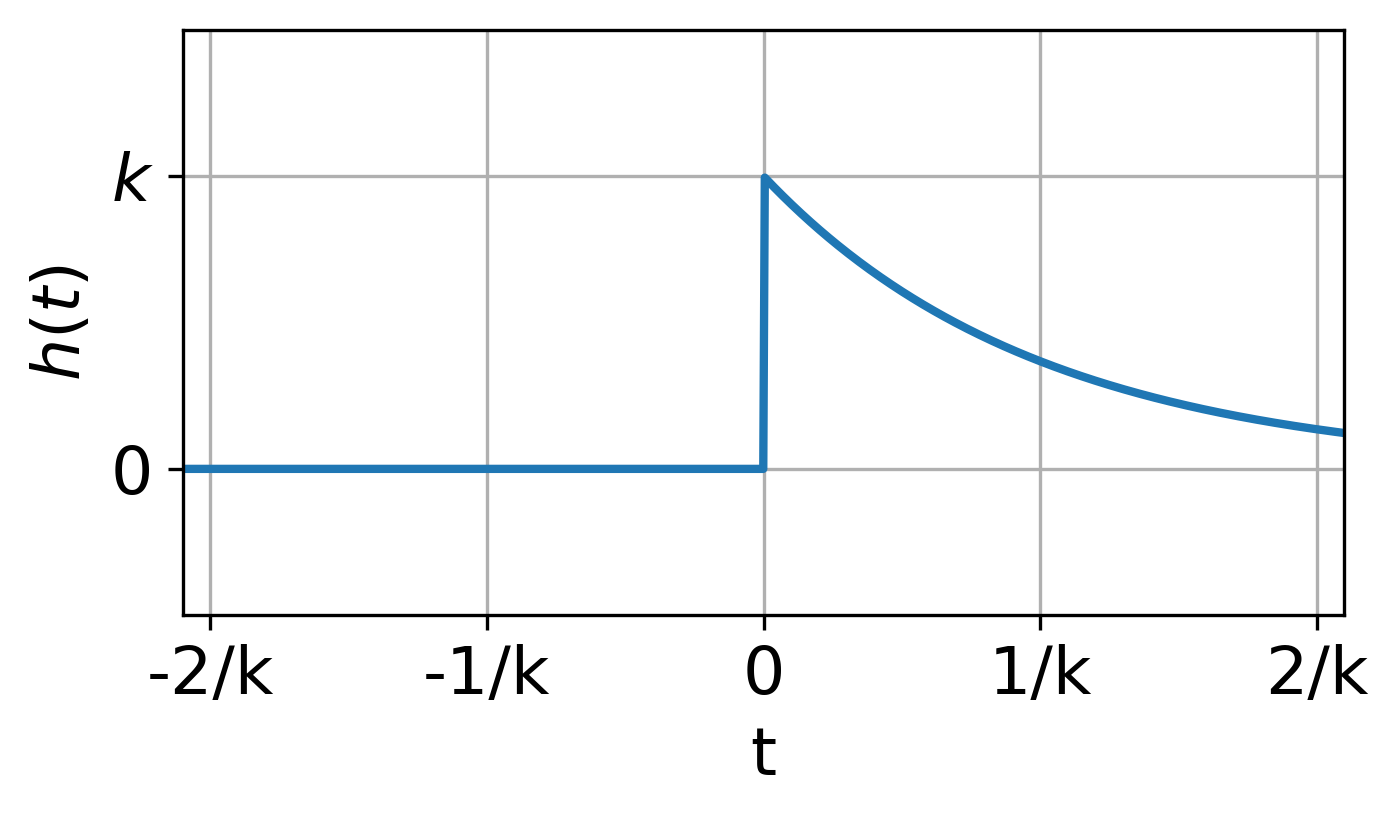
\includegraphics[width=\textwidth/5]{thermo_impulse_response}
		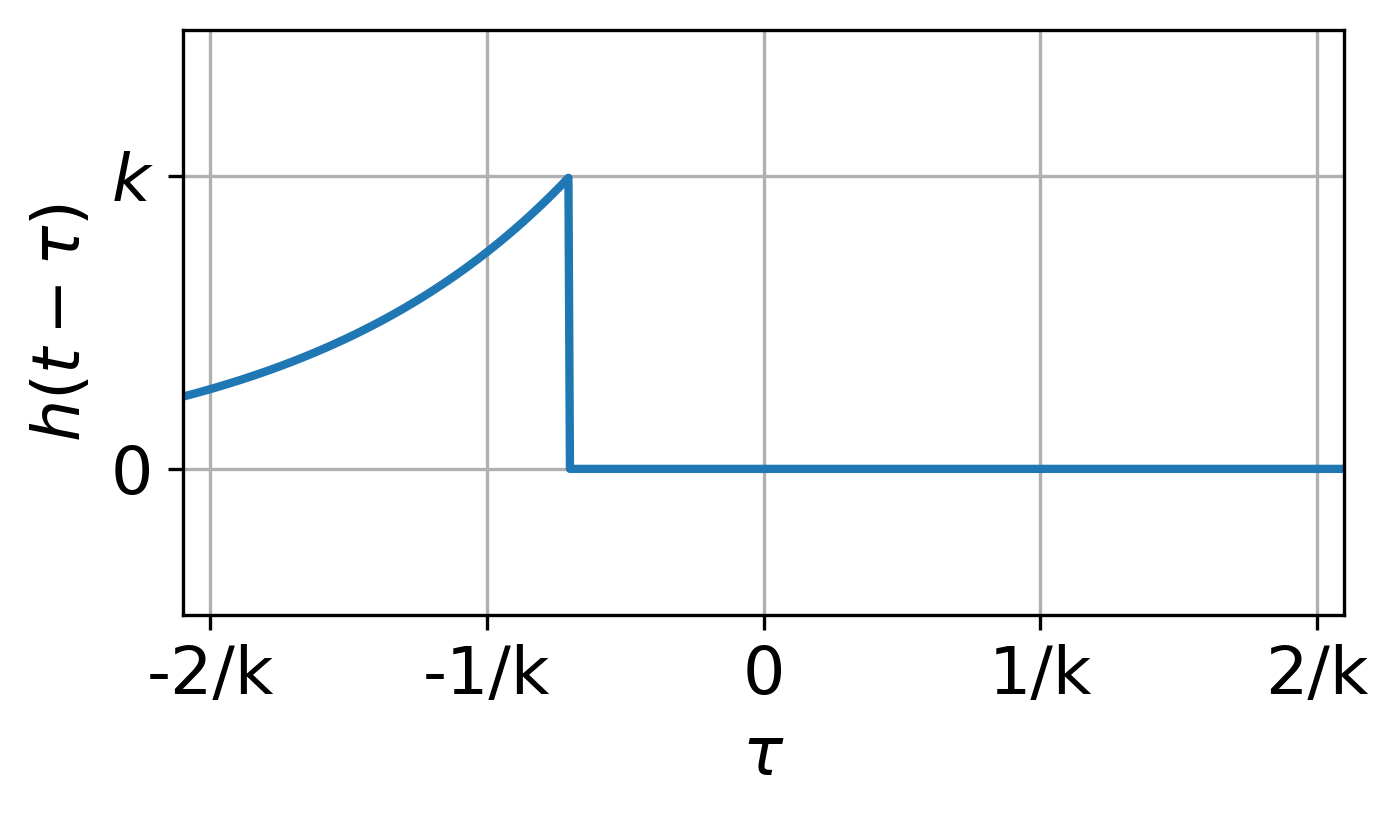
\includegraphics[width=\textwidth/5]{thermo_impulse_response_reversed_case1}
		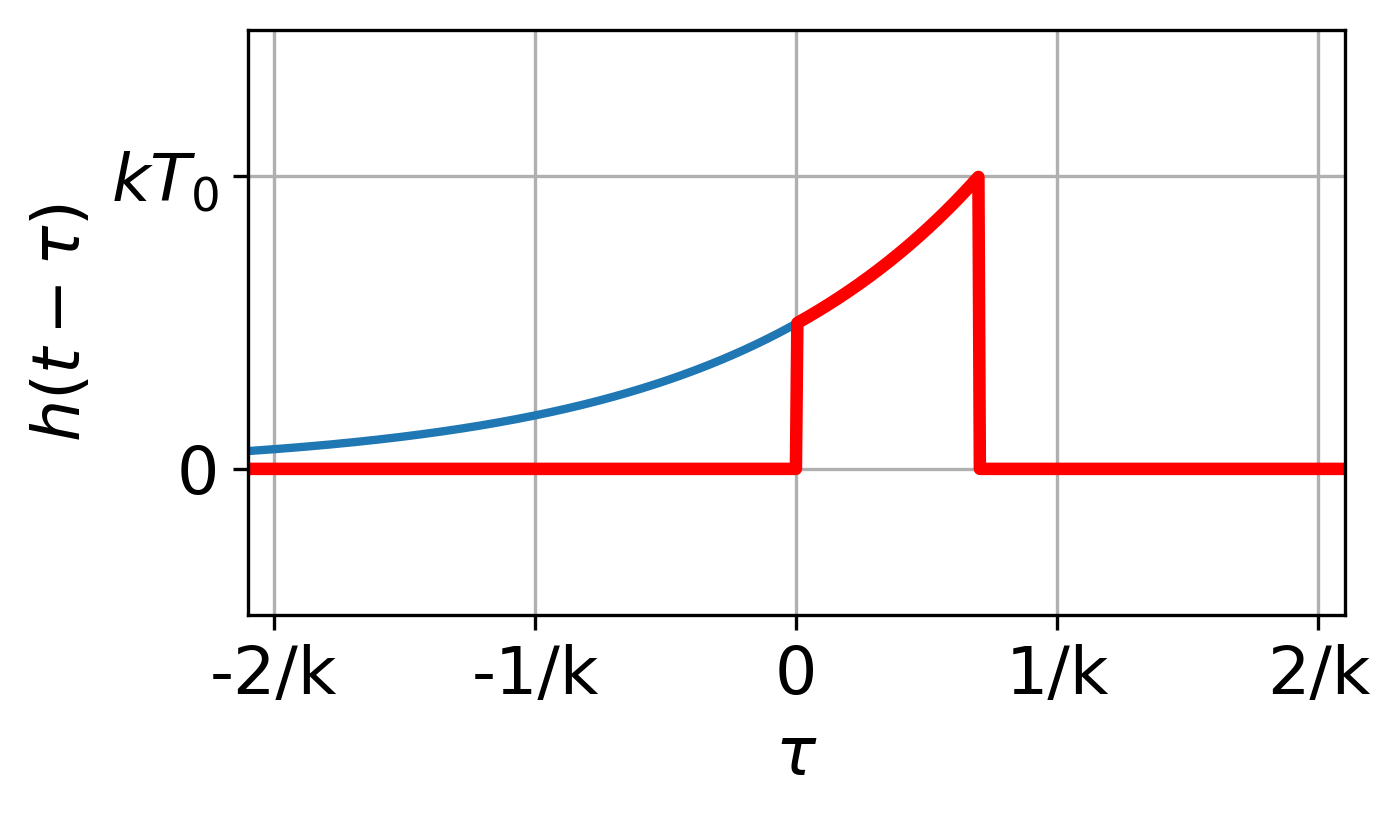
\includegraphics[width=\textwidth/5]{thermo_impulse_response_reversed_case2b}
		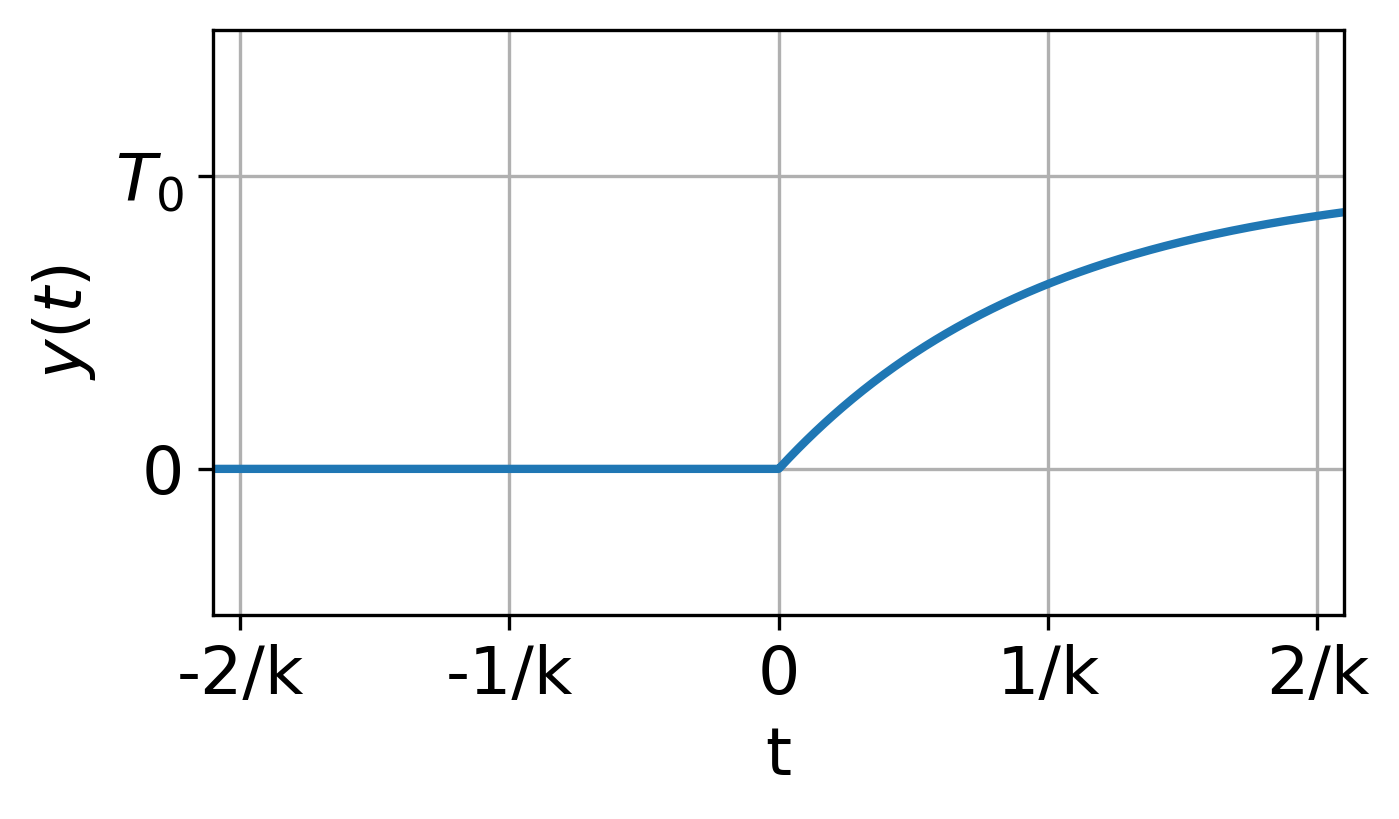
\includegraphics[width=\textwidth/5]{thermo_step_response}\\
		Temporal length of the output = length of input + length of $h(t)$.
		
		\newpage
		\section{Computing convolutions by hand.}
			\begin{itemize}
				\item Sketch functions.\\
				\item Identify cases/intervals\\
				\item Solve integral as a function of $ t $.
			\end{itemize}
		
		\section{Properties of the convolution.}
		Commutative: $x(t) * y(t) = y(t) * x(t)$\\
		Associative: $x(t) * h_1(t) * h_2(t) = x(t)*(h_1(t)*h_2(t))$\\
		Distributive: $x(t) * h_1(t) + x(t) * h_2(t) = x(t)*(h_1(t)+h_2(t))$
		
		\section{Frequency response.}
		\[
			x(t) = e^{j 2\pi f_0 t} \rightarrow \boxed{\text{H(f)}} \rightarrow e^{j 2\pi f_0 t} \cdot H(f_0)
		\]
		\[
			\begin{split}
				x(t) * h(t) & = \int_{-\infty}^{\infty} h(\tau) \cdot e^{j 2\pi f_0 (t-\tau)}~d\tau \\
				& = e^{j 2\pi f_0 t} \int_{-\infty}^{\infty} h(\tau) \cdot e^{- j 2\pi f_0 \tau}~d\tau
			\end{split}
		\]
		$H(f)$: frequency response. The frequency response is the Fourier transform of the impulse response.
		\[
			H(f) = \int_{-\infty}^{\infty} h(\tau) \cdot e^{-j2\pi f \tau}~d\tau = \int_{-\infty}^{\infty} h(t) \cdot e^{-j2\pi ft}~dt
		\]
		
		\section{Constructing periodic signals.}
			\begin{align*}
				x_0(t) &= a_0 + \sum_{k=1}^{n} a_k \cos(k \omega_0 t) + \sum_{k=1}^{n} b_k \sin(k \omega_0 t)\\
				&=\sum_{n=-N}^{N} X_n e^{j n \omega_0 t}
			\end{align*}
		
		\section{Synthesis and analysis equations.}
		A non-pathological periodic function with period $T_0$ can be expressed as
		\[
			x(t) = \sum_{n=0}^{\infty} a_n \cos(n \omega_0 t) + \sum_{n=1}^{\infty} b_n \sin(n \omega_0 t)
		\]
		with\\
		$\qquad a_0 = \frac{1}{T_0} \int_{<T_0>} x(t)~dt = \frac{1}{T_0} \int_{0}^{T_0} x(t)~dt = \frac{1}{T_0} \int_{-T_0/2}^{T_0/2} x(t)~dt$\\
		$\qquad a_n = \frac{2}{T_0} \int_{<T_0>} x(t) \cdot \cos(n \omega_0 t)~dt$\\
		$\qquad b_n = \frac{2}{T_0} \int_{<T_0>} x(t) \cdot \sin(n \omega_0 t)~dt$\\
		$a_0$ is the mean value. $\cos(n \omega_0 t)$ are even functions of $t(x(t) = x(-t))$. $\sin(n \omega_0 t)$ are odd functions of $t(x(t) = -x(-t))$.\\
		A signal $ x(t) $ can always be decomposed in an even and an odd component:
		\[
			x(t) = x_{\text{even}}(t) + x_{\text{odd}}(t)
		\]
		
		\section{Complex Fourier series.}
		Since
		\[
			\cos(n \omega_0 t) = \frac{1}{2} e^{-j n \omega_0 t} + \frac{1}{2} e^{j n \omega_0 t}
		\]
		and
		\[
			\sin(n \omega_0 t) = \frac{j}{2} e^{-j n \omega_0 t} - \frac{j}{2} e^{j n \omega_0 t},
		\]
		we can rewrite the Fourier series as
		\[
			x(t) = \sum_{n=0}^{\infty} a_n \cos(n \omega_0 t) + \sum_{n=1}^{\infty} b_n sin(n \omega_0 t) = \sum_{n=-\infty}^{\infty} X_n \cdot e^{j n \omega_0 t}
		\]
		with
		\[
			X_n = \frac{1}{T_0} \int_{<T_0>} x(t) \cdot e^{-j n \omega_0 t}~dt
		\]
		
		\section{Symmetry property.}
		For real-valued signals:
		\[
			X_n = X_{-n}^*
		\]
		Real part is even function of $n$.\\
		Imaginary part is odd function of $n$.\\
		Amplitude $\lvert X_n \rvert$ is even function.\\
		Phase is odd.\\
		Altogether this is called Hermitian symmetry.
		
		\section{Differentiation.}
		\[
			x(t) \rightarrow \boxed{\frac{d}{dt}} \rightarrow \mathcal{H}[x(t)] = \frac{dx(t)}{dt} = \dot{x}(t)
		\]
		Per definition:
		\[
			h(t) = \dot{\delta}(t)
		\]
		Thus:
		\[
			\mathcal{H}[x(t)] = x(t) * \dot{\delta}(t) = \int_{-\infty}^{\infty} x(\tau) \cdot \dot{\delta}(t - \tau)~dt = \dot{x}(t)
		\]
			\begin{align*}
				e^{jk\omega_0 t} \rightarrow &\boxed{\frac{d}{dt}} \rightarrow jk\omega_0 \cdot e^{jk\omega_0 t}\\
				X_l e^{jl\omega_0 t} + X_k e^{jk\omega_0 t} \rightarrow &\boxed{\frac{d}{dt}} \rightarrow jl\omega_0 X_l e^{jl\omega_0 t} + jk\omega_0 X_k e^{jk\omega_0 t}\\
				\sum_{k=-\infty}^{\infty} X_k e^{jk\omega_0 t} \rightarrow &\boxed{\frac{d}{dt}} \rightarrow \sum_{k=-\infty}^{\infty} jk\omega_0 X_k e^{jk\omega_0 t}
			\end{align*}
		Thus the derivative of a complex Fourier series is another one with new coefficients
		\[
			X_k^{\prime} = jk\omega_0 X_k
		\]
		
		\section{Response of LTI system to periodic signal.}
		\[
			\sum_{k=-\infty}^{\infty} X_k e^{jk\omega_0 t} \rightarrow \boxed{\begin{matrix}h(t)\\H(\omega)\end{matrix}} \rightarrow \sum_{k=-\infty}^{\infty} H(k\omega_0) \cdot X_k e^{jk\omega_0 t}
		\]
		Thus the response of a LTI system to a periodic signal is another periodic signal with the same fundamental period and coefficients
		\[
			\tilde{X}_k = H(k\omega_0) \cdot X_k
		\]
		E.g. differentiation: $ H(\omega) = j\omega $.
		
		\section{Parseval's theorem.}
			\begin{align*}
				P &= \frac{1}{T_0} \int_{0}^{T_0} {\lvert x(t) \rvert}^2~dt = \frac{1}{T_0} \int_{0}^{T_0} x(t) \cdot x(t)^*~dt\\
				&= \sum_{n=-\infty}^{\infty} X_n^* \cdot X_n = \sum_{n=-\infty}^{\infty} {\lvert X_n \rvert}^2
			\end{align*}
		For trigonometric series:
			\begin{align*}
			P &= \frac{1}{T_0} \int_{0}^{T_0} {\lvert x(t)\rvert}^2~dt = \frac{1}{T_0} \int_{0}^{T_0} x(t) \cdot x(t)^*~dt\\
			&= a_0^2 + \frac{1}{2} \sum_{n=1}^{\infty} a_n^2 + \frac{1}{2} \sum_{n=1}^{\infty} b_n^2
			\end{align*}
		
		\section{Time and frequency.}
		As the signal becomes shorter in the time domain, we need higher frequencies to synthesize it.
			\begin{align*}
				\text{Short/concentrated in time} &\leftrightarrow \text{long/extended in frequency}\\
				\text{Long/extended in time} &\leftrightarrow \text{short/concentrated in frequency}
			\end{align*}
		
		\section{Fourier transform.}
			\begin{align*}
				\text{Fourier Transform:}~&X(f) = \int_{-\infty}^{\infty}{x(t)\cdot e^{-j2\pi ft}~dt}\\
				\text{Inverse Fourier Transform:}~&x(t) = \int_{-\infty}^{\infty}{X(f)\cdot e^{j2\pi ft}~df}
			\end{align*}
		
		\section{Duality.}
		Given the Fourier transform pair
		\[
			\F\left\{x(t)\right\} = X(f)
		\]
		we also have the following one:
		\[
			\F\left\{X(t)\right\} = x(-f)
		\]
		
		\section{Convolution and product theorems.}
			\begin{center}\begin{tabular}{l l}
					Time domain & Frequency domain\\
					\hline
					$ x(t) \ast h(t) $ & $ X(f) \cdot H(f) $\\
					$ x(t) \cdot y(t) $ & $ X(f) \ast Y(f) $
			\end{tabular}\end{center}
		$ Y(f) = H(f) \cdot X(f) $\\
		Fourier transforms are slight extensions of Fourier series:
			\begin{align*}
				x(t) &= \int_{-\infty}^{\infty}{X(f)\cdot e^{j2\pi ft}~df} \rightarrow \boxed{\begin{matrix}h(t)\\H(f)\end{matrix}}\\
				&\rightarrow y(t) = \int_{-\infty}^{\infty} H(f)\cdot X(f)\cdot e^{j2\pi ft}~df
			\end{align*}
		
		\section{Energy of signal after going through system.}
		Parseval's theorem:
		\[
			E = \int_{-\infty}^{\infty} \left|x(t)\right|^2~dt = \int_{-\infty}^{\infty} \left|X(f)\right|^2~df
		\]
		\[
			x(t)~\text{with}~E_x \rightarrow \boxed{\begin{matrix}h(t)\\H(f)\end{matrix}} \rightarrow y(t)~\text{with}~E_y
		\]
		\[
			E_y = \int_{-\infty}^{\infty}{\left|y(t)\right|^2~dt} = \int_{-\infty}^{\infty}{\left|Y(f)\right|^2~df}
		\]
		First route: calculate $ y(t)=x(t)\ast h(t) $ and continue from there.\\
		Second route: $ Y(f)=H(f)\cdot X(f)$, thus
		\[
			E_y = \int_{-\infty}^{\infty}{\left|H(f)\right|^2\left|X(f)\right|^2~df}
		\]
		
		\section{Filters.}
		Low-pass Butterworth filter example:
		\[
			H_{\text{Butter}}(f) = \frac{1}{B_n\left(j\cdot \frac{f}{f_c}\right)}
		\]
		where $ B_n(s) $ are the Butterworth polynomials of order $ n $.\\
		E.g. $ B_2(s) = s^2 + \sqrt{2}s + 1 $.\\
		In general:
		\[
			\left|H_{\text{Butter}}(f)\right|^2 = \frac{1}{1+\left(\frac{f}{f_c}\right)^{2n}}
		\]
		At $ f_c $ (or $ f_1 $, $ f_2 $) we have $ \left| H(f_c)\right|^2 = \frac{1}{2} $.
			\begin{align*}
				\text{Higher order filter} &\rightarrow \text{sharper in frequency domain}\\
				&\rightarrow \text{longer impulse response}\\
				&\rightarrow \text{more complexity}
			\end{align*}
		
		\section{Fourier transform vs DFT.}
		\textbf{Fourier Transform.}\\
		Physical world: continuous time signals $ x(t) $  for $ t \in \left[-\infty,\infty\right] $.\\
			\begin{align*}
				X(f) &= \int_{-\infty}^{\infty}{x(t)\cdot e^{-j2\pi ft}~dt}\\
				x(t) &= \int_{-\infty}^{\infty}{X(f)\cdot e^{j2\pi ft}~df}
			\end{align*}
		$ X(f) $ is continuous, $ f\in \left[-\infty,\infty\right] $.\\
		\textbf{Discrete Fourier Transform.}\\
		Typical digital world: discrete time signals $ x[n] $ for $ n=0,1,...,N-1 $.
			\begin{align*}
				X[k] &= \sum_{n=0}^{N-1}{x[n]e^{-j2\pi \frac{k\cdot n}{N}}}\\
				x[n] &= \frac{1}{N}\sum_{k=0}^{N-1}{X[k]e^{j2\pi \frac{k\cdot n}{N}}}
			\end{align*}
		$ X[k] $ is discrete. Discrete angular frequencies $ 0,\frac{2\pi}{N},\frac{2\pi\cdot2}{N},...,\frac{2\pi\cdot(N-1)}{N} $.
		
		\section{Discrete Fourier Transform.}
		Very often $ x[n] $ are samples of a continuous time signal:
		\[
			x[n] = x(n\cdot T_s)
		\]
		In those cases, the discrete frequencies correspond to continuous time frequencies
		\[
			f_k = \frac{k}{N}\cdot F_s = \frac{k}{N\cdot T_s} = \frac{k}{T_{\text{meas}}}
		\]
		Frequency resolution:
		\[
			\Delta f=\frac{F_s}{N}=\frac{1}{N\cdot T_s}=\frac{1}{T_{\text{meas}}}
		\]
		DFT treats signals as periodic: we take $ N $ samples of a continuous time signal. Since we do not know what happens before or after, we can assume that the signal is periodic.\\
		First $ N/2 $ values of DFT: positive frequencies.\\
		Second $ N/2 $ values of DFT: negative frequencies.\\
		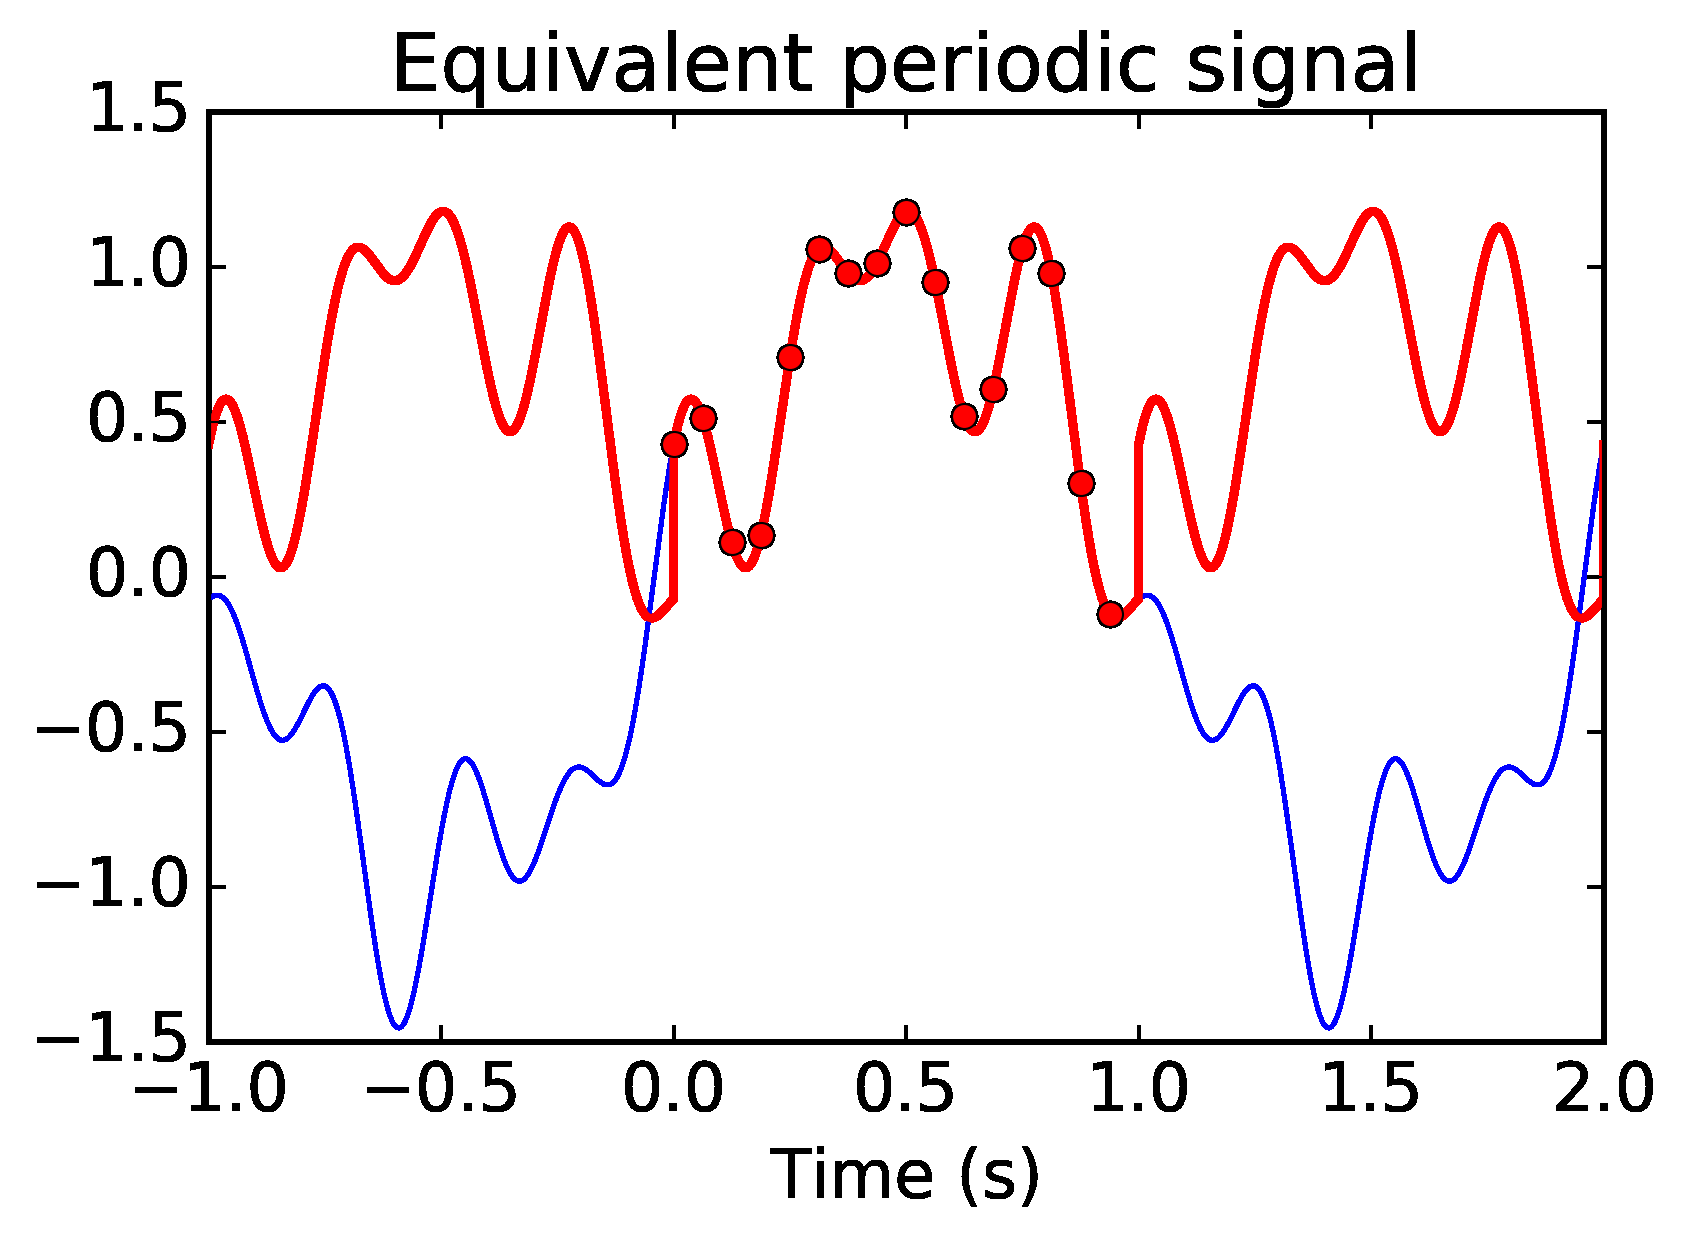
\includegraphics[width=\textwidth/5]{dft-equivalent-signal}\\
		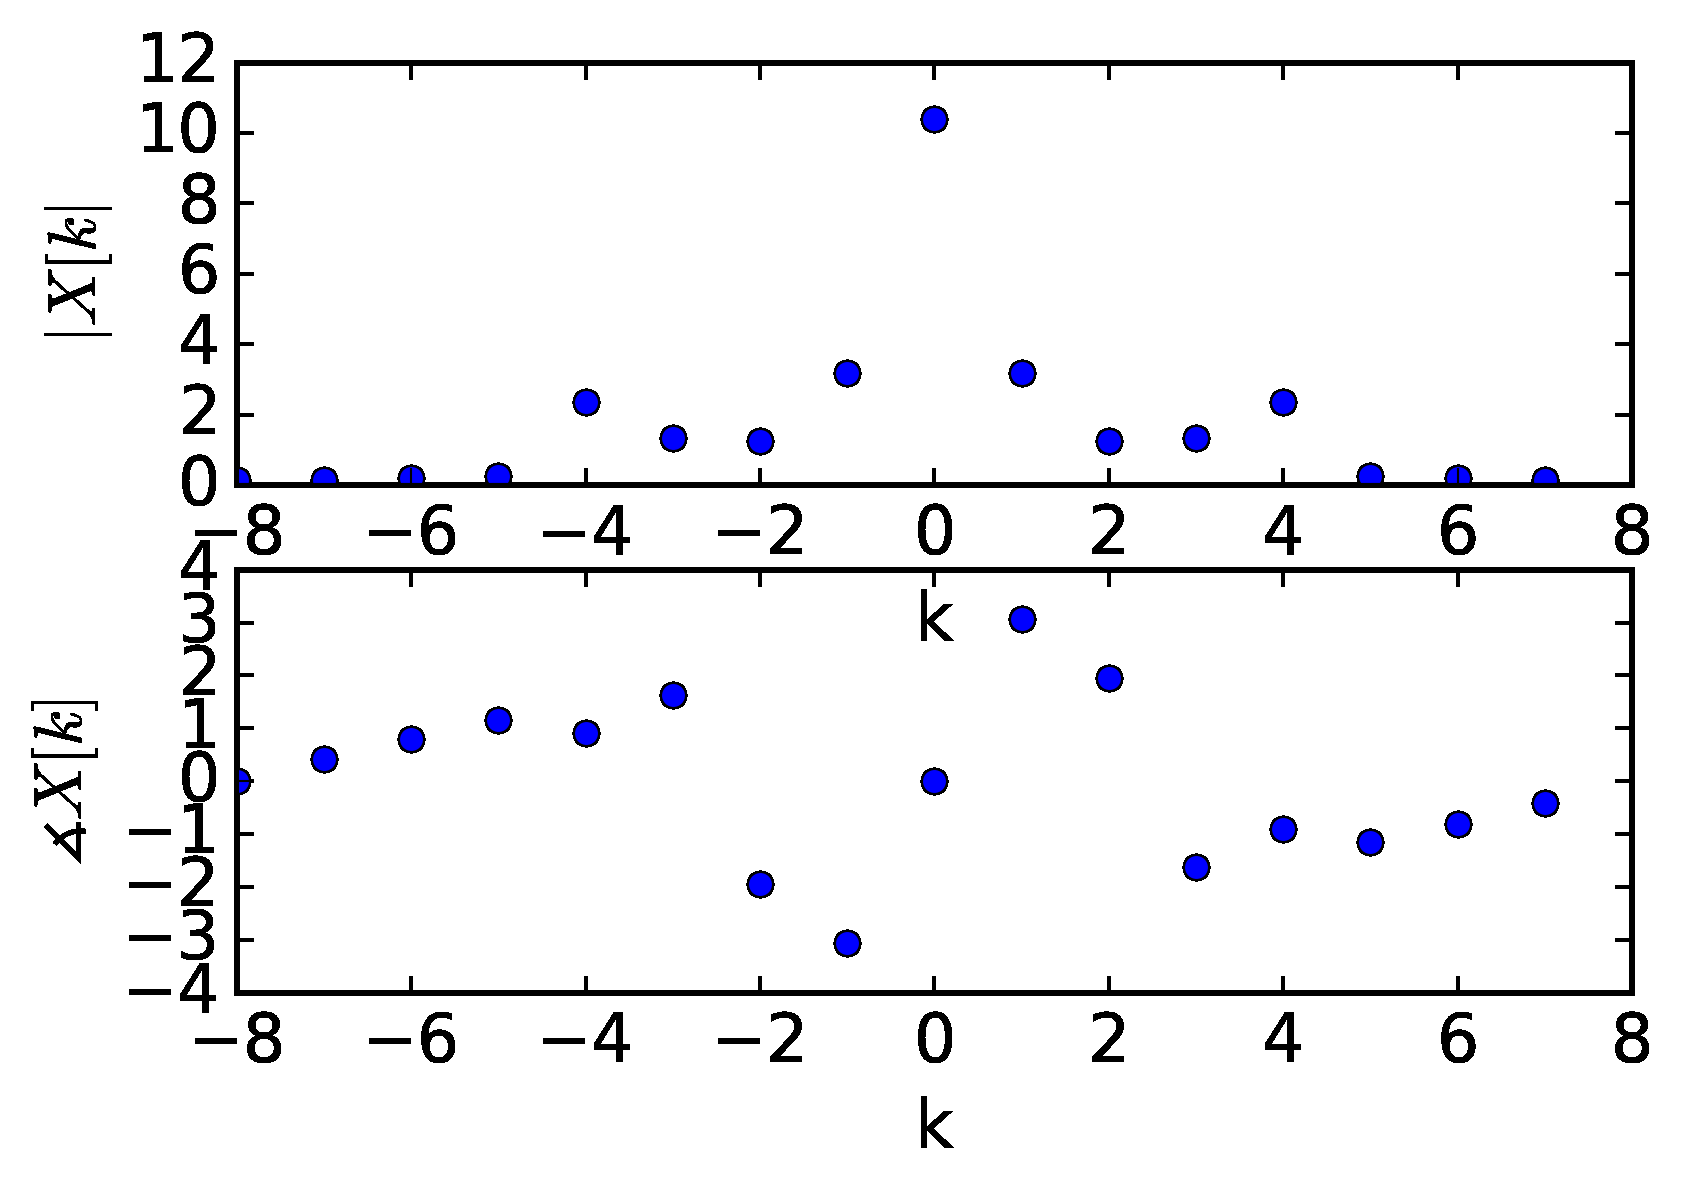
\includegraphics[width=\textwidth/5]{dft-result}\\
		
		\section{DFT vs FFT.}
		The Fast Fourier Transform is a family of algorithms to efficiently compute the DFT: number of operations for DFT according to formula is $ \mathcal{O}\left(N^2\right) $; number of operations for FFT is $ \mathcal{O}\left(N\cdot\log N\right) $.\\
		
		\section{Aliasing.}
		Causes different signals to become indistinguishable (or aliases to one another) when sampled.\\
		Possible aliases for $ x(t)=\cos\left(2\pi \cdot4.5\cdot t\right) $ sampled at $ F_s = 15~\text{Hz} $:\\
		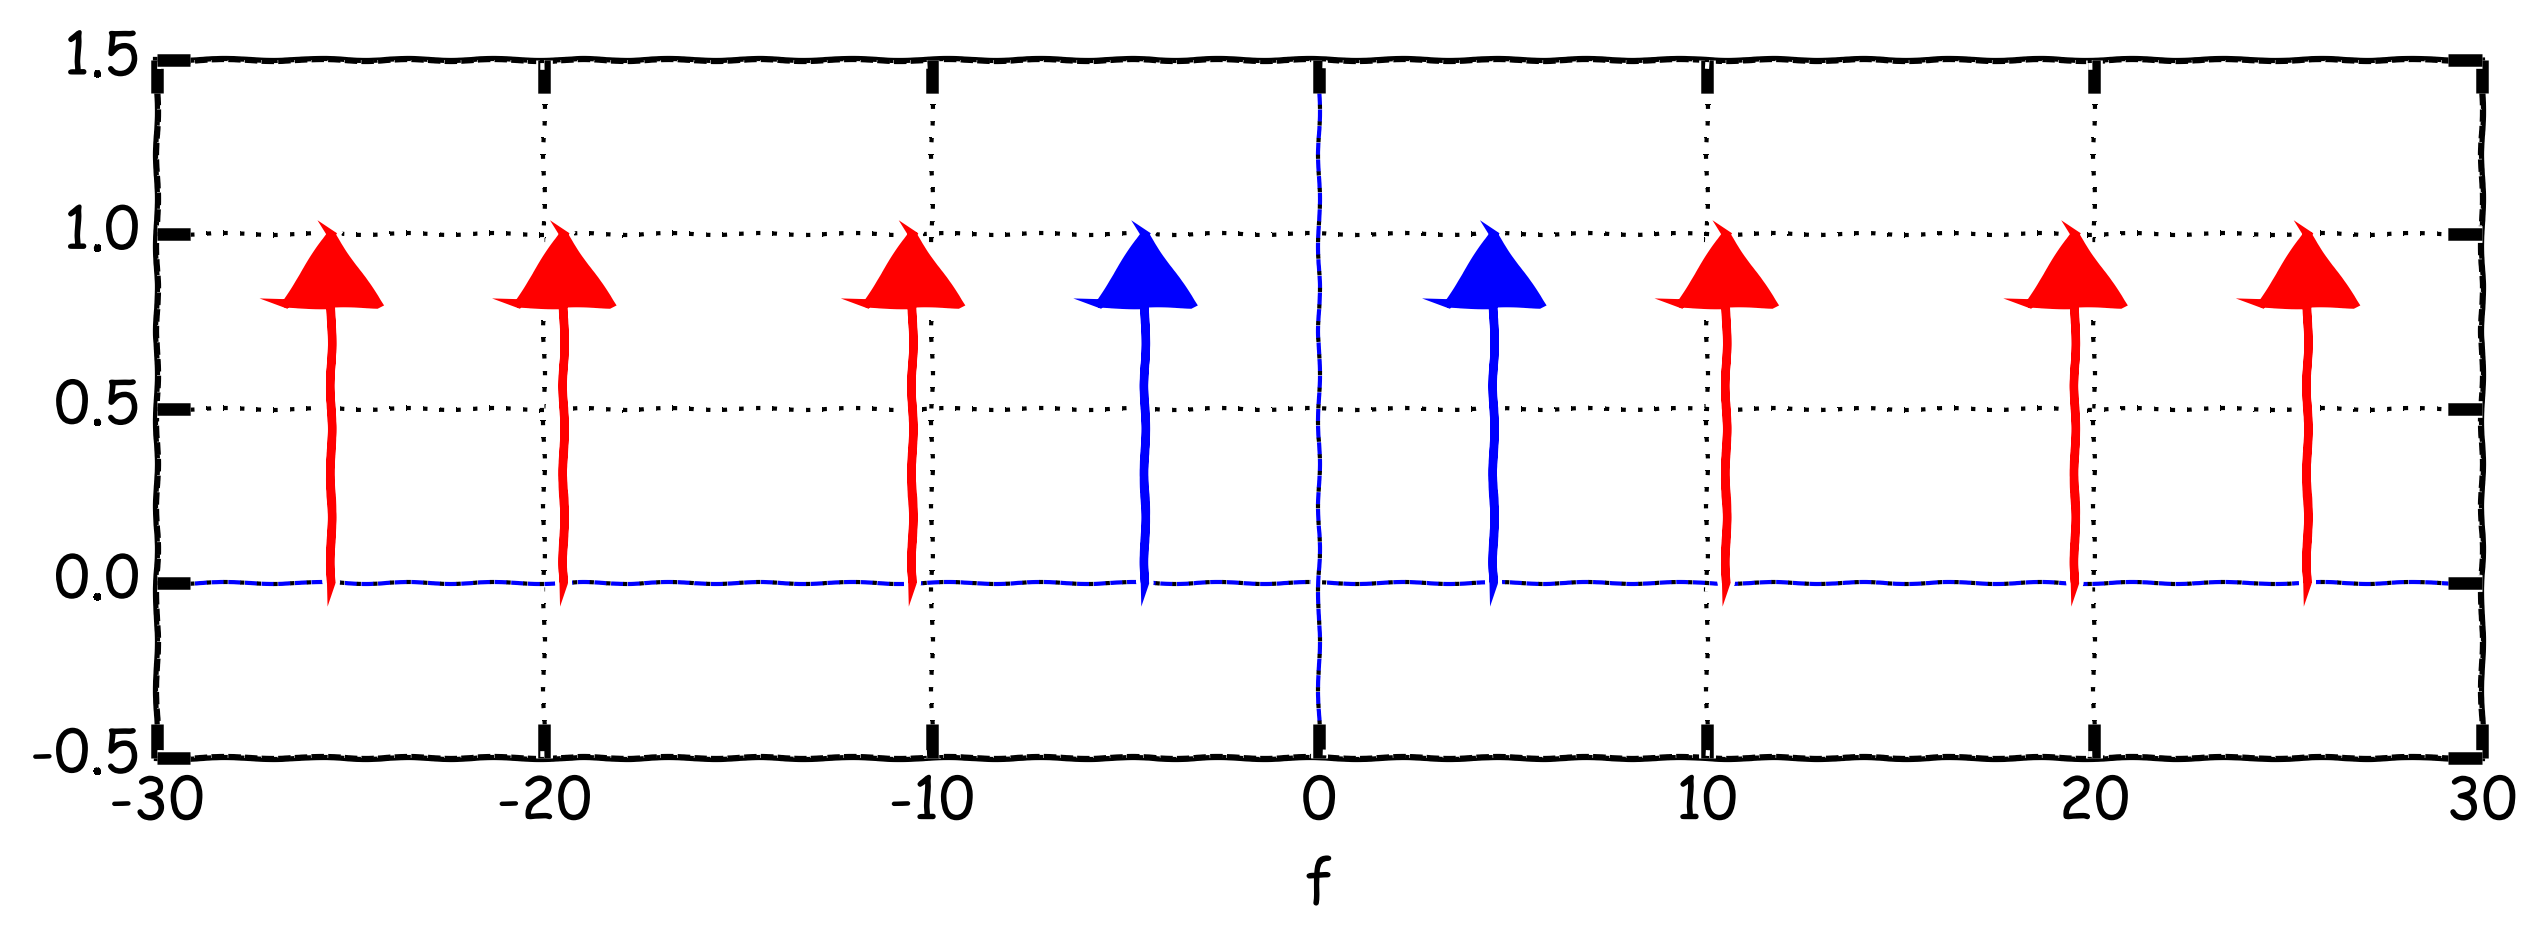
\includegraphics[width=\textwidth/5]{possible-aliases}\\
		
		\section{Nyquist Theorem.}
		To perfectly reconstruct a signal, the sampling frequency $ F_s $ needs to be at least twice the highest frequency $ W $ of a given signal:
		\[
			F_s>2\cdot W
		\]
		
		\section{Simple sampling scheme: Sample and Hold.}
		Sample and Hold: retain values of signal at instants
		\[
			t_n = n\cdot T_s
		\]
		During sampling, this operation gives the Digital to Analog Converter (DAC) time to do the quantization of the signal.
		
		\section{Ideal sampling.}
		We can model sampling as multiplying a continuous time signal $ x(t) $ with a train of Dirac-deltas:
			\begin{align*}
				x_s(t) &= x(t)\cdot \sum_{n=-\infty}^{\infty}{T_s\cdot \delta\left(t-n\cdot T_s\right)}\\
				&= T_s\sum_{n=-\infty}^{\infty}{x\left(n\cdot T_s\right)\cdot \delta\left(t-n\cdot T_s\right)}
			\end{align*}
			\begin{align*}
				&\boxed{x_s(t) = x(t)\cdot T_s\sum_{n=-\infty}^{\infty}{\delta\left(t-n\cdot T_s\right)}} \overset{\F}{\leftrightarrow} \boxed{X_s(f)=X(f)\ast\sum_{k=-\infty}^{\infty}{\delta\left(f-k\cdot F_s\right)}}\\
				&\boxed{x_s(t)=T_s\sum_{n=-\infty}^{\infty}{x\left(n\cdot T_s\right)\cdot \delta\left(t-n\cdot T_s\right)}} \overset{\F}{\leftrightarrow} \boxed{X_s(f)=\sum_{k=-\infty}^{\infty}X\left(f-k\cdot F_s\right)}
			\end{align*}
		
		\section{Ideal reconstruction.}
		Given a properly sampled signal $ \left(F_s>2\cdot W\right) $ we can reconstruct the original perfectly using a Sinc interpolation (essentially the same as using a low pass filter):
		\[
			x(t) = \sum_{n=-\infty}^{\infty}{x[n]\cdot \sinc\left(\frac{t-n\cdot T_s}{T_s}\right)}
		\]
		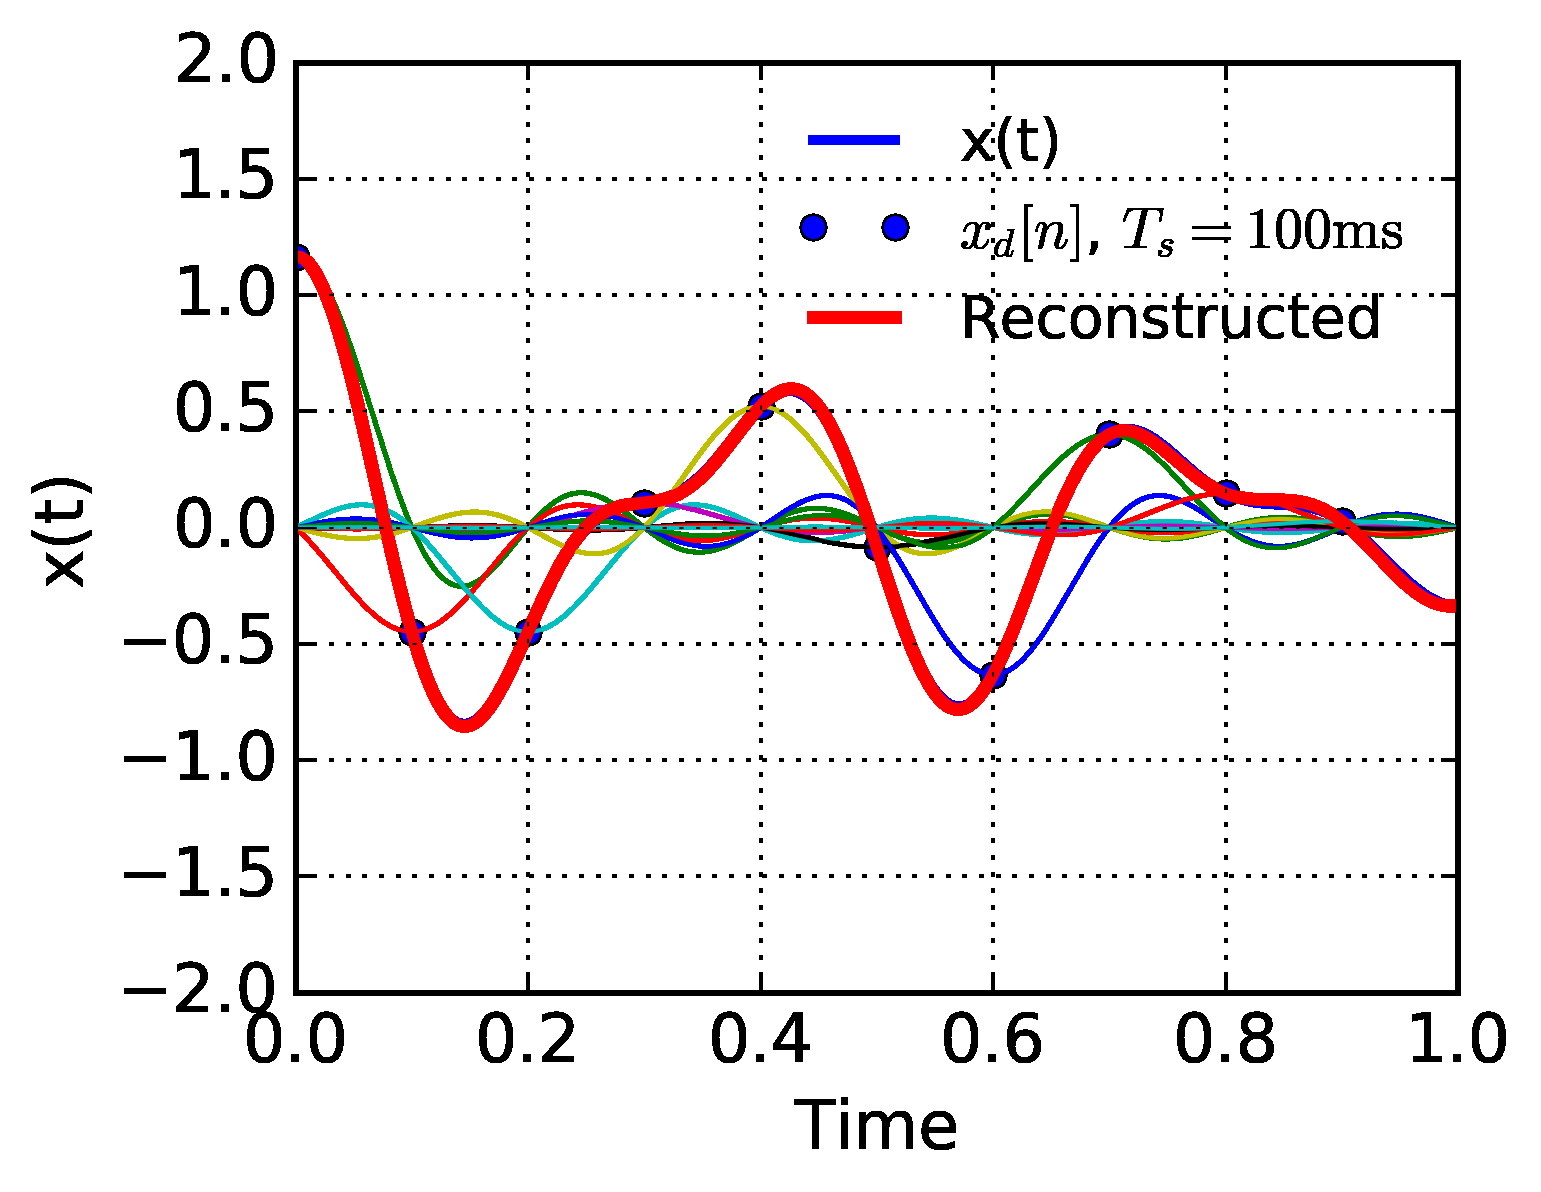
\includegraphics[width=\textwidth/5]{reconstruction}\\
			\begin{align*}
				x[n]\rightarrow\boxed{\text{DAC}}\underset{X(f)\ast\sum_{k=-\infty}^{\infty}{\delta\left(f-k\cdot F_s\right)}}{\xrightarrow{T_s\sum_{n=-\infty}^{\infty}{x[n]\delta\left(t-nT_s\right)}}}\boxed{\text{Ideal LPF}}\xrightarrow{\sum_{n=-\infty}^{\infty}{x[n]\sinc\left(t-nT_s\right)}=x(t)}
			\end{align*}
		
		
		\newpage
		\part*{Various Fourier transforms.}
		
		\section{From Fourier series to Fourier transform.}
			\begin{align*}
				x(t)&=\sum_{n=-\infty}^{\infty}{X_n\cdot e^{jn\omega_0t}}\\
				X_n&=\frac{1}{T_0}\int_{<T_0>}{x(t)\cdot e^{-jn\omega_0t}~dt}
			\end{align*}
		Move $ \frac{1}{T_0} $ to $ x(t) $, use $ \omega_0=2\pi f_0 $, and rewrite.
			\begin{align*}
				x(t)&=\sum_{n=-\infty}^{\infty}{X[n]\cdot e^{j2\pi nf_0t}\frac{1}{T_0}}\\
				X[n]&=\int_{<T_0>}{x(t)\cdot e^{-j2\pi nf_0t}~dt}
			\end{align*}
		Write $ X[n] $ as a continuous function of $ f $ and use $ f_0=\frac{1}{T_0} $.
			\begin{align*}
				x(t)&=\sum_{n=-\infty}^{\infty}{X(nf_0)\cdot e^{j2\pi nf_0t}f_0}\\
				X(nf_0)&=\int_{<T_0>}{x(t)\cdot e^{-j2\pi nf_0t}~dt}
			\end{align*}
		Now: we let $ T_0 \rightarrow \infty $, or $ f_0 \rightarrow 0 $; we call this $ df $; use $ f=n\cdot f_0 $; and the summation becomes an integral.
			\begin{align*}
				\text{Inverse Fourier Transform:}~&x(t) = \int_{-\infty}^{\infty}{X(f)\cdot e^{j2\pi ft}~df}\\
				\text{Fourier Transform:}~&X(f) = \int_{-\infty}^{\infty}{x(t)\cdot e^{-j2\pi ft}~dt}
			\end{align*}
		
		\section{Fourier transform of Dirac delta.}
		\[
			\F\left\{\delta(t)\right\}=\int_{-\infty}^{\infty}{\delta(t)\cdot e^{-j2\pi ft}~dt}
		\]
		Apply shifting property.
		\[
			\F\left\{\delta(t)\right\}=\int_{-\infty}^{\infty}{\delta(t)\cdot e^{-j2\pi ft}~dt} = 1
		\]
		Did we know this?
		\[
			x(t)\rightarrow\boxed{\delta(t)}\rightarrow x(t)
		\]
		We knew the expression of the frequency response:
			\begin{align*}
				H(f)&=\int_{-\infty}^{\infty}{h(t)\cdot e^{-j2\pi ft}~dt}\\
				&=\int_{-\infty}^{\infty}{\delta(t)\cdot e^{-j2\pi ft}~dt}=1
			\end{align*}
		
		\section{Fourier transform of a delay.}
			\begin{align*}
				\F\left\{\delta(t-\tau)\right\}&=\int_{-\infty}^{\infty}{\delta(t-\tau)\cdot e^{-j2\pi ft}~dt}\\
				&=\int_{-\infty}^{\infty}{\delta(t-\tau)e^{-j2\pi ft}~dt}\\
				&=e^{-j2\pi f\tau}
			\end{align*}
		
		\section{Duality example.}
			\begin{align*}
				X(f)&=\delta(F)\\
				x(t)=\int_{-\infty}^{\infty}{X(f)e^{j2\pi ft}~df}&=\int_{-\infty}^{\infty}{\delta(f)\cdot e^{j2\pi ft}~df}=1\\
				1&\xLeftrightarrow[\F^{-1}]{\F}\delta(f)
			\end{align*}
		What is the Fourier transform of
		\[
			x_1(t)=\frac{1}{10+j2\pi t}
		\]
		From the Fourier transform pair table:
		\[
			\F\left\{e^{-\alpha t}\cdot u(t)\right\}=\frac{1}{\alpha +j2\pi f}=X(f)
		\]
		Take $ \alpha=10 $, then we have $ x_1(t)=X(f) $, therefore
			\begin{align*}
				\F\left\{x_1(t)\right\}=\F\left\{X(f)\right\}&=e^{-\alpha(-f)}\cdot u(-f)\\
				\F\left\{\frac{1}{10+j2\pi t}\right\}&=e^{10f}\cdot u(-f)
			\end{align*}
		
		\section{Fourier Transform theorems.}
			\begin{align*}
				&\qquad\text{Time domain}\quad&\text{Frequency domain}\\
				\text{Superposition}\quad&a_1x_1(t)+a_2x_2(t)&a_1X_1(f)+a_2X_2(f)\\
				\text{Time delay}\quad&x(t-t_0)&e^{-j2\pi ft_0}X(f)\\
				\text{Scaling}\quad&x(a\cdot t)&\frac{1}{\left|a\right|}X\left(\frac{f}{a}\right)\\
				\text{Time reversal}\quad&x(-t)&X(-f)\\
				\text{Frequency translation}\quad&x(t)\cdot e^{j2\pi f_0t}&X(f-f_0)\\
				\text{Modulation}\quad&\cos{2\pi f_0t\cdot x(t)}&\frac{1}{2}X(f-f_0)+\frac{1}{2}X(f+f_0)\\
				\text{Differentiation}\quad&\frac{d}{dt}x(t)&j2\pi fX(f)\\
				\text{Integration}\quad&\int_{-\infty}^{t}x(\alpha)d\alpha&\frac{1}{j2\pi f}X(f)+\frac{1}{2}X(0)\delta(f)
			\end{align*}
		
		\section{Fourier transform of unit pulse.}
		\[
			\F\left\{\Pi\left(\frac{t}{A}\right)\right\}=A\sinc(f\cdot A)
		\]
		
		\section{Fourier transform of sinc.}
		\[
			x(t)=\sinc(2Wt)
		\]
		Use duality to write
			\begin{align*}
				\F\left\{A\cdot\sinc(t\cdot A)\right\} =\Pi\left(-\frac{f}{A}\right)&=\Pi\left(\frac{f}{A}\right)\\
				\frac{1}{2W}\F\left\{2W\cdot\sinc(2Wt)\right\} &=\frac{1}{2W}\Pi\left(\frac{f}{2W}\right)\\
				\F\left\{\sinc(2Wt)\right\}&=\frac{1}{2W}\Pi\left(\frac{f}{2W}\right)
			\end{align*}
		
		\section{Fourier transform of train of deltas.}
		To find the Fourier transform of
		\[
			T_s\sum_{n=-\infty}^{\infty}{\delta\left(t-n\cdot T_s\right)}
		\]
		we are going to use Fourier series:
			\begin{align*}
				T_s\sum_{n=-\infty}^{\infty}{\delta\left(t-n\cdot T_s\right)} &= \sum_{k=-\infty}^{\infty}{X_k\cdot e^{j2\pi kF_st}}\\
				&= \sum_{k=-\infty}^{\infty}{e^{j2\pi kF_st}}
			\end{align*}
		Thus
			\begin{align*}
				\F\left\{T_s\sum_{n=-\infty}^{\infty}{\delta\left(t-n\cdot T_s\right)}\right\} &= \F\left\{\sum_{k=-\infty}^{\infty}{e^{j2\pi kF_st}}\right\}\\
				&= \sum_{k=-\infty}^{\infty}{\delta\left(f-kF_s\right)}
			\end{align*}
		
		\newpage
	\end{multicols}
\end{document}













